\documentclass[a4paper, 12pt]{memoir}
\usepackage[danish]{babel}
\usepackage[utf8]{inputenc}
\renewcommand{\danishhyphenmins}{22}
\usepackage[T1]{fontenc}
\usepackage{amsmath}
\usepackage{amssymb}
\newcommand{\Cov}{\textup{Cov}}
\newcommand{\xdot}{x_{\cdot}}
\usepackage{SASnRdisplay}
\usepackage{mathtools}
\newcommand{\Rroom}[2]{\mathbb R^{#1 \times #2}}
\renewcommand{\i}{^{-1}}
\newcommand{\tr}{\textup{tr}}
\usepackage{bm}
\usepackage{tikz}
\definecolor{blue1}{rgb}{0.7,0.8,1}
\definecolor{blue2}{rgb}{0.6,0.8,1}
\definecolor{blue3}{rgb}{0.7,0.9,1}
\definecolor{blue4}{rgb}{0.6,0.7,1}

\definecolor{red1}{rgb}{1,0.5,0.7}
\definecolor{red2}{rgb}{1,0.7,0.75}
\definecolor{red3}{rgb}{1,0.7,0.5}
\definecolor{red4}{rgb}{1,0.8,0.7}
\definecolor{red5}{rgb}{1,0.5,0.5}

\definecolor{gron}{rgb}{0,0.6,0}

\newcommand{\bigzero}{\mbox{\normalfont\Large\bfseries 0}}
\newcommand{\rvline}{\hspace*{-\arraycolsep}\vline\hspace*{-\arraycolsep}}


\begin{document}

Lad $\omega$ være en amerikaner. Definer
\begin{align*}
F_i(\omega)&= \textup{ værdien af faktoren } i \textup{`te faktor for } \omega\\
D(\omega)&= \textup{ dødsårsag for } \omega\\
L(\omega)&= \textup{  dødsalder for } \omega
\end{align*}
I det kommende undertrykkes afhængigheden af $\omega$. 
\subsection{Faktorsandsynligheder}

Vi har blandt andet brug for størrelserne
\begin{gather*}
P(F_i\in f), \textup{ for forskellige mængder } f\in \mathcal F_i\\
P(F_{i_1}\in f_1, F_{i_2}\in f_2, \dots F_{i_n}\in f_n) \textup{ for } f_i, i=1, \dots, n
\end{gather*}
hvor $f_i$ er mængder der giver mening for deres tilhørende faktor. I filerne i mappen Factor\_frequencies ligger filer af typen.
\begin{align*}
 i_1 \textup{`te faktor} \quad& \cdots&  i_n\textup{`te faktor} \qquad& 	\textup{freq}\\
f_1^0 \quad & \cdots& f_n^0 \qquad&  P(F_{i_1}\in f_1^0, F_{i_2}\in f_2^0, \dots F_{i_n}\in f_n^0)\\
f_1^0 \quad & \cdots& f_n^1 \qquad&  P(F_{i_1}\in f_1^0, F_{i_2}\in f_2^0, \dots F_{i_n}\in f_n^1)\\
\vdots\quad &\cdots &\vdots \qquad &\vdots\\
f_1^0 \quad & \cdots& f_n^{n_k} \qquad&  P(F_{i_1}\in f_1^0, F_{i_2}\in f_2^0, \dots F_{i_n}\in f_n^{n_k})\\
\vdots\quad &\cdots &\vdots \qquad &\vdots\\
f_1^{n_1} \quad & \cdots& f_n^{n_k} \qquad& P(F_{i_1}\in f_1^{n_1}, F_{i_2}\in f_2^{n_2}, \dots F_{i_n}\in f_n^{n_k})
\end{align*}
Alternativt kan man skrive $F=(F_{i_1}, \dots , F_{i_n})$
\subsection{Incidents}

Dernæst har vi sandsynlighederne for at dø af en dødsårsag i løbet af et år.
\begin{gather*}
p_d(l)=P(D=d, L\leq l \mid L> l-1), d\in \mathcal D, l\in \mathbb R_+
\end{gather*}
hvor $\mathcal D$ er en mængde af alle dødsårsager i programmet. For beregning, kender vi $p_d(l)$ som stykvis konstant funktion på mængderne
\begin{equation*}
l_1,l_2, \dots, l_{22}=[0,1), [1,5), [5,10),\dots, [95,100), [100,\infty)
\end{equation*}
Vi er interesserede i vektoren
\begin{alignat*}{4}
p_d(l_1)\quad & p_d(l_2)\quad & \cdots \quad & p_d(l_{22})
\end{alignat*}
hvor vi, med den lidt misbrugte notation $p_d(l_i)$, mener $p_d(l)$ for et $l\in l_i$. Disse estimeres med
\begin{equation*}
p_d(l_i)\leftarrow \frac{\textup{antal amerikanere døde af } d \textup{ i aldersgruppen } l_i \textup{ i år } Y_1}{\textup{antal amerikanere i aldersgruppen } l_i \textup{ i år } Y_2 }=:\frac{a_{di}}{a_i}
\end{equation*}
(Lige nu har vi $Y_1=2014, Y_2=2013$). Filerne af formen \emph{ICDcode.txt} indikerer et $d$ med deres titel og indholdet er
\begin{alignat*}{4}
a_{d1} \quad &a_{d2} \quad &\cdots \quad &a_{d22}  
\end{alignat*}
Og filen \emph{population.txt} indeholder
\begin{alignat*}{4}
a_{1} \quad &a_{2} \quad &\cdots \quad &a_{22}  
\end{alignat*}

\subsection{Risk ratios}
Lad $F_1, \dots, F_k$ være nogle faktorer. Risk ratios i dette program fortolkes som
\begin{align*}
\textup{RR}_{d}(f):=\frac{P\bigl(D=d, L \leq l \mid L>l-1, (F_1, \dots, F_k)\in f \bigr)}{P\bigl(D=d, L \leq l \mid L>l-1, (F_1, \dots, F_k)\in f_0\bigr)}
\end{align*}
Egentlig skulle der et $f_0$ på i notationen for $\textup{RR}_{d}(f)$, for at indikere at det er riskratio med hensyn til baselinen $f_0$. Det er en antagelse, at riskratioen ikke afhænger af $l$. Risk ratioerne er kendt for en mængde af faktorinddelinger $f\in \mathcal F$. Vi kræver mere eller mindre at $\mathcal F$ kan skrives på formen
\begin{equation*}
\mathcal F=\mathcal F_1 \times \mathcal F_2 \times \cdots \mathcal F_k
\end{equation*}
hvor 
\begin{equation*}
\mathcal F_i = \{f_1^0, f_1^1, \dots, f_1^{n_i}\}
\end{equation*}
og så er de kodet ved hjælp af 
\begin{align*}
 i_1 \textup{`te faktor} \quad& \cdots&  i_k\textup{`te faktor} \qquad& 	\textup{RR}\\
f_1^0 \quad & \cdots& f_k^0 \qquad&  RR_d((f_1^0, \dots, f_k^0))\\
f_1^0 \quad & \cdots& f_k^1 \qquad&  RR_d((f_1^0, \dots, f_k^1))\\
\vdots\quad &\cdots &\vdots \qquad &\vdots\\
f_1^0 \quad & \cdots& f_k^{n_k} \qquad&  RR_d((f_1^0, \dots, f_k^{n_k}))\\
\vdots\quad &\cdots &\vdots \qquad &\vdots\\
f_1^{n_1} \quad & \cdots& f_k^{n_k} \qquad& RR_d((f_1^{n_1}, \dots, f_k^{n_k}))
\end{align*}

\section{Udregning}
I første omgang vil vi gerne udregne
\begin{align}
P\bigl(D=d, L\leq l \mid L>l-1, F=f\bigr), \, \textup{for } f\in \mathcal F \label{firstpart}
\end{align}
hvor $F$ er en vektor af faktorer og $\mathcal F$ er den endelige mængder af faktorsammensætninger. \eqref{firstpart} kan senere(i javascript-delen) bruges til at udregne
\begin{equation}
P\bigl(D=d, L\leq l \mid L>l-1, F=f_{\textup{personal}}\bigr)\label{lastpart}
\end{equation}
hvor $f_{\textup{personal}}$ ikke (nødvendigvis) ligger i $\mathcal F$.
Det gøres ved
\begin{align}
\eqref{firstpart}=\frac{\textup{RR}_{d}(f)}{\sum_{f\in \mathcal F} RR_d(f)\cdot P(F=f)}p_d(l) \label{rr_calc}
\end{align}

Der er dog nogle forhindringer før vi bare kan stoppe tallene fra filerne ind i \eqref{rr_calc}.
\begin{itemize}
\item
Vi ikke har nok information til at kende $P(F=f), f\in \mathcal F$ 100\%.
\item
Vi har flere riskratio filer for samme $d$. 
\item
Hvordan man skal tage højde for alders specifikke riskratios og alders specifikke $P(F=f)$'er
\end{itemize}
Lad os tage dem i voksende sværhedsgrad

\subsection{Flere risk ratio filer}
Hvis vi der er to riskratiofiler baseret på to vektorer af faktorer $F^1$, $F^2$ og to tilhørende krydsmængder, $\mathcal F^1$ og $\mathcal F^2$, så ville den mest rigtige måde at kombinere dem på være
\begin{align}
P\bigl(D=d&, L\leq l \mid L>l-1, (F^1,F^2)=(f^1,f^2)\bigr)\label{trueRR}\\
&=\frac{g(\textup{RR}_{d}(f^1),\textup{RR}_{d}(f^2))}{\sum_{f^1,f^2\in \mathcal F^1\times \mathcal F^2} g(\textup{RR}_{d}(f^1),\textup{RR}_{d}(f^2))\cdot P((F^1,F^2)=(f^1,f^2))}p_d(l)\nonumber
\end{align}
hvor $g$ er en passende interaktionsfunktion. Hvis $F^1$ og $F^2$ er uafhængige og $g(x,y)=x\cdot y$, kan man dog skrive det som
\begin{align}
P\bigl(D=d&, L\leq l \mid L>l-1, (F^1,F^2)=(f^1,f^2)\bigr)\label{prodRR}\\
&=\frac{\textup{RR}_{d}(f^1)}{\sum_{f^1\in \mathcal F^1} RR_d(f^1)\cdot P(F^1=f^1)}\frac{\textup{RR}_{d}(f^2)}{\sum_{f^2\in \mathcal F^2} RR_d(f^2)\cdot P(F^2=f^2)}p_d(l)\nonumber
\end{align}
Fordelen ved \eqref{prodRR} er, at man kan lægge et tallene 
\begin{equation*}
\frac{\textup{RR}_{d}(f^1)}{\sum_{f^1\in \mathcal F^1} RR_d(f^1)\cdot P(F^1=f^1)}, f^1\in \mathcal F^1
\end{equation*}
i en fil og tallene
\begin{equation*}
\frac{\textup{RR}_{d}(f^2)}{\sum_{f^2\in \mathcal F^2} RR_d(f^2)\cdot P(F^2=f^2)}, f^2\in \mathcal F^2
\end{equation*}
i en anden fil og tallene
\begin{equation*}
p_d(l_i), \, i=1, \dots, 22
\end{equation*}
i en tredje fil. Selvom betingelserne for at bruge \eqref{prodRR} ikke er helt er opfyldt, kan det måske alligevel være en god ide at bruge den. 

\subsection{Vi kender ikke $\bm{P(F=f), f\in \mathcal F}$}
Her tænkes $\mathcal F$ som den mængde hvor vi kender $\textup{RR}_d(f)$ hvis og kun hvis $f\in \mathcal F$.

Der er flere slags udfordringer her. 
\begin{enumerate}
\item
Det hænder at vi kun kender
\begin{equation*}
P(F=f), f \in \mathcal F'
\end{equation*}
hvor $\mathcal F'\not\supseteq \mathcal F$.
\item
Vi har $\mathcal F=\mathcal F_1 \times \mathcal F_2$ og $F=(F_1,F_2)$, hvor $F_1$ og $F_2$ er hver deres faktor. Her hænder det at vi kun kender
\begin{equation*}
P(F_i=f_i), f_i\in \mathcal F_i 
\end{equation*}
for $i=1,2$ og altså ingenting om den simultane fordeling af $(F_1,F_2)$
\item
Vi har $\mathcal F= \mathcal F_1\times \mathcal F_2\times F_3$ og $F=(F_1,F_2,F_3)$. Det hænder, at vi kun kender
\begin{align*}
P((F_1,F_2)&=(f_1,f_2)), \, f_1\in \mathcal F_1, f_2\in \mathcal F_2\\
P((F_1,F_3)&=(f_1,f_3)), \, f_1\in \mathcal F_1, f_3\in \mathcal F_3
\end{align*}
\item
Vi har $\mathcal F= \mathcal F_1$ og $F=F_1$. Det hænder, at vi kender
\begin{align*}
P((F_1,F_2)&=(f_1,f_2)), \, f_1\in \mathcal F_1, f_2\in \mathcal F_2
\end{align*}
men ikke (umiddelbart)
\begin{align*}
P(F_1&=f_1), \, f_1\in \mathcal F_1
\end{align*}
så vi så om sige har for meget
\item
Vi har $\mathcal F= \mathcal F_1$ og $F=F_1$. Det hænder, at vi slet ikke kender noget til
\begin{align*}
P(F_1\in f)
\end{align*}
\end{enumerate}
Problemerne findes også i flere flere dimensioner og med kombinationer. 

\subsubsection*{En løsning af problem 4}
Vi laver en funktion som marginaliserer, dvs
\begin{equation*}
P(F_1=f_1)=\sum_{f_2\in \mathcal F_2} P((F_1,F_2)=(f_1,f_2))
\end{equation*}

\subsubsection*{En løsning af problem 1}

Hvis vi laver en funktion, som laver transformationen
\begin{align*}
w:\{P(F=f_1), &P(F=f_2), \dots, P(F=f_n)\}\\&\mapsto \{P(F=f_1'), P(F=f_2'), \dots, P(F=f_k')\}
\end{align*}
kan vi løse det første problem. Hvis vi antager 
\begin{equation}
\bigcup_{i=1}^nf_i\subseteq\bigcup_{j=1}^k f_j'\label{condFaktorCoverage}
\end{equation}
kan man lave løsningen
\begin{align*}
P(F=f_j')=&w\bigl( P(F=f_1), P(F=f_2), \dots, P(F=f_n)\bigr)\\
&=\sum_{i=1}^n\frac{P(F=f_i) \cdot |f_i\cap f_j'|}{|f_i|}
\end{align*}
hvor $|\cdot|$ repræsenterer et mål. Det vil dog nok altid være muligt at bruge Lebesguemålet eller tællemålet og nogle gange kan man måske være nødt til at bruge en mikstur af de to. Det ses foreksempel ved rygning, hvor der er en kategori, der hedder 0 cigaretter. Betingelsen \eqref{condFaktorCoverage} er nødvendig for at $P(F=f_j'), j=1,\dots, k$ summer til 1(det er nemlig antaget at $P(F=f_i), i=1, \dots ,n$ summer til 1). 




\subsubsection*{En løsning af problem 2,3 og 5}
For at løse problem 2,3 og 5 kan man bruge tilpasning af marginaler. Man har den ønskede fordeling
\begin{equation*}
P(F=f), f\in \mathcal F
\end{equation*}
hvor $F=(F_1, \dots, F_k)$ og $\mathcal F = \mathcal F_1 \times \cdots \times \mathcal F_k$, og man kender
\begin{align*}
P(F^1=f^1)&, f^1\in \mathcal F^1\\
&\vdots\\
 P(F^m=f^m)&, f^m\in \mathcal F^m
\end{align*}
hvor $\mathcal F^l=\mathcal F_{i^l_1}\times \mathcal F_{i^l_2}\times \cdots \times \mathcal F_{i^l_{r_l}}$. Man starter med en standard uniformfordeling
\begin{equation*}
p(f)=\frac{1}{\#\mathcal F},\,  f\in \mathcal F 
\end{equation*}
som estimater for $P(F=f)$. Dernæst \emph{tilpasser man med marginalen} $\mathcal F^1$
\begin{equation*}
p^{ny}(f)=p(f)\frac{P(F^1=f^1(f))}{\sum_{f': f^1(f')=f^1(f)}p(f')}
\end{equation*}
og derefter med marginalen $\mathcal F^2, \mathcal F^3$ og så videre (indtil man når til hvad?). 

\subsubsection{Forskellige credibilities}
Vi har mængder, $f\in \mathcal F$, for hvilke vi vil finde $P(F=f)$. $F$ kan her skrives $(F_i)_{i\in I}$, hvor $I$ er en mængde i $\{1, \dots, n\}$. Vi kender da `binnede' fordelinger af $(F_i)_{i\in I_j}$ for $j=1, \dots, k$, hvor $I_j$ også er mængder i  $\{1, \dots, n\}$. Credibility-scoren er en funktion $c: \{I_j\}_{j=1, \dots, k} \to \mathbb R_+$. De binnede fordelinger, der indgår i konstruktionen $P(F=f)$ er
\begin{equation*}
\Bigl\{            (F_i)_{i\in I_j} \mid I_j\cap I\neq \emptyset \wedge \bigl(\not\exists k : I\cap I_j\subseteq I\cap I_k \wedge c(I_k)>c(I_j)  \bigr)           \Bigr\}
\end{equation*}•


\subsection{Aldersspecifikke $\bm{P(F=f)}$'er eller riskratioer}
I princippet burde alle ovenstående udregninger laves separat for alle aldersgrupper. Det gøres også, og der er nogle genveje. Definer $A$ til at være den stokastiske variabel der angiver alderen på personen. De nye faktorsandsynlighedsfiler har specificerende kolonner ved
\begin{align*}
 i_1 \textup{`te faktor} \quad& \cdots&  i_n\textup{`te faktor}\quad & \textup{aldersgr.}\\
f_1^0 \quad & \cdots& f_n^0 \qquad& A_1 \\
f_1^0 \quad & \cdots& f_n^1 \qquad&  A_1\\
\vdots\quad &\cdots &\vdots \qquad &\\
f_1^0 \quad & \cdots& f_n^{n_k} \qquad&  A_1 \\
\vdots\quad &\cdots &\vdots \qquad &\\
f_1^{n_1} \quad & \cdots& f_n^{n_k} \qquad& A_h\\
\end{align*}
og freq kolonnen indeholder
\begin{align*}
& \textup{freq}\\
&P(F_{i_1}\in f_1^0, F_{i_2}\in f_2^0, \dots F_{i_n}\in f_n^0\mid A\in A_1)\\
&P(F_{i_1}\in f_1^0, F_{i_2}\in f_2^0, \dots F_{i_n}\in f_n^1\mid A\in A_1)\\
&\vdots\\
& P(F_{i_1}\in f_1^0, F_{i_2}\in f_2^0, \dots F_{i_n}\in f_n^{n_k}\mid A\in A_1)\\
&\vdots\\
&P(F_{i_1}\in f_1^{n_1}, F_{i_2}\in f_2^{n_2}, \dots F_{i_n}\in f_n^{n_k}\mid A\in A_h)
\end{align*}
Det vil sige, at freq-kolonnen skal summe til $h$. Når man konstruerer $P(F=f)$, bør man konstruere 

\section{Javascript delen}
Til hver cause hører noget data på formen
\begin{align*}
d, \bigl(p_d(l_i)\bigr)_{i=1, \dots, 22} \textup{ dataframe}, \textup{risk ratio data}_d
\end{align*}
hvor $d$ bare er en string, $\bigl(p_d(l_i)\bigr)_{i=1, \dots, 22}$ er en data frame udskrevet som liste og risk ratio data'et har formen
\begin{equation*}
(\textup{Risk ratio datagruppe})^d_1,(\textup{Risk ratio datagruppe})^d_2,\dots,  (\textup{Risk ratio datagruppe})^d_{n_d}
\end{equation*}
En risk ratio datagruppe - indekseret ved $(j,d)$ - består af
\begin{equation*}
(\textup{norm}^{j,d}(l_i))_{i=1, \dots, 22}, (\textup{risk ratio dataframe}_i^{j,d})_{i=1, \dots, k_{j,d}}, g_{j,d}
\end{equation*}
hvor $(\textup{norm}^j(l_i))_{i=1, \dots, 22}$ er en liste af 22 tal som normaliserer for hver af de 22 aldersgrupper, $\textup{list of risk ratio dataframes}$ er en liste af risk ratio dataframes udskrevet som lister og $g_{j,d}$ er en string, som siger hvilken interaktion der mellem $(j,d)$ dataframesne. En risk ratio dataframe for en faktor $F^{i,j,d}$ har formen
\begin{equation*}
(r^{i,j,d}(f))_{f\in \mathcal F^{i,j,d}}
\end{equation*}
hvor $\mathcal F^{i,j,d}$ er en endelig mængde af faktor levels. Dette $r$ er blot en diskretisering af den underliggende riskfaktor funktion
\begin{equation*}
R^{i,j,d}(\psi), \psi \in  \Psi^{i,j,d}
\end{equation*}
hvor $\Psi^{i,j,d}$ er en mængde af alle tænkelige værdier af faktoren $F^{i,j,d}$, og derfor kan den være uendelig. Vi vil lave en \emph{polating} funktion, pol, til at evaluere funktionen
\begin{equation}
R^{i,j,d}(\psi)=\textup{pol}((r^{i,j,d}(f))_{f\in \mathcal F^{i,j,d}}, \psi) \label{polating}
\end{equation}

Lad nu $\psi$ være alle en persons faktorværdier, og lad $\phi^{i,j,d}$ være vektoren af faktorer der er relevante for den $(i,j,d)$'te risk ratio fil, dvs. en delvektor af $\psi$. Lad $a$ være en vilkårlig alder og lad $l(a)$ være den af de 22 alderskategorier, som $a$ falder i. Så defineres

\begin{equation}
P_{d}(a,\psi)=P_{d}(a) \cdot \prod_{j=1}^{n_d} \frac{g_{j,d}(R^{1,j,d}(\psi^{1,j,d}),  \dots , R^{k_{j,d},j,d}(\psi^{k_{j,d},j,d}) )}{\textup{norm}^{j,d}(l(a))}\label{pda_calculation}
\end{equation}

hvor $P_d(a)$ er `afdiskretiseringen' af $p_d(l)$. Det kunne måske defineres som
\begin{equation*}
P_d(a)=\max\bigl(1,\textup{pol}(\bigl(p_d(l_i)\bigr)_{i=1, \dots, 22}, a)\bigr)
\end{equation*}

Størrelsen $P_d(a,\psi)$ tænkes at være det samme som \eqref{lastpart}, dvs.
\begin{equation}
P_d(a,\psi) =P\bigl(D=d, L\leq a \mid L>a-1, F=\psi\bigr)\label{base_prob}
\end{equation}

\subsection{Kombinationer af $P_d(a)$'er}

Vi definerer nu
\begin{equation*}
p(a,\psi)=\sum_{d\in \mathcal D}p_d(a,\psi)
\end{equation*}
hvor $\mathcal D$ er mængden af alle dødsårsager. Hvis \eqref{base_prob} faktisk gælder, er
\begin{equation*}
p(a,\psi)=P(L\leq a \mid L>a-1, F=\psi\bigr)
\end{equation*}


\subsubsection{Liste over mest interessante kombinationer}
Lad nu $\tilde{\mathcal D}  \subseteq \mathcal D$ være en vilkårlig delmængde af dødsårsagerne. Alle de følgende størrelser kan varieres ved at tilføje $d\in  \tilde{\mathcal D}$ og/eller $L\in [a,b]$ til betingningen
\begin{itemize}
\item
Forventet levealder
\begin{equation*}
E[L\mid \psi] = \sum_{a=0}^\infty a \cdot p(a, \psi)\prod_{b=0}^{a-1} (1-p(b,\psi))
\end{equation*}
\item
Forventet antal år mistet til sygdom $d$
\begin{equation*}
E[L\mid \psi, D\in \mathcal D\setminus \{d\}]-E[L\mid \psi]
\end{equation*}
\item
Sandsynligheden for at dø af $d$
\begin{equation*}
P(D=d\mid \psi)= \sum_{a=0}^\infty  p_d(a, \psi)\prod_{b=0}^{a-1} (1-p(b,\psi))
\end{equation*}
\item
Ens overlevelseskurve
\begin{align*}
(P(L\geq a \mid \psi))_{a\in \mathbb N_0} = \biggl(\prod_{b=0}^{a-1} (1-p(b,\psi))\biggr)_{a\in \mathbb N_0}
\end{align*}
\end{itemize}

\subsection{Forklare døden ved hjælp af ens faktorer}

Vi vil nu også lave en optimal $\psi$-værdi som man kan måle brugerens $\psi$ op imod. Dette er dog en udfordring, fordi en faktor som forårsager en sygdom kan hæmme fremkomsten af en anden sygdom. Det gælder foreksempel rygning, lungekræft og Parkinson's. Vi definerer derfor $\psi_0$ så $\psi_0^{i,j,d}$ minimerer $R^{i,j,d}(\cdot)$. Det vil sige at i en lungekræftssammenhæng har $\psi_0$ rygning på 0, mens i en Parkinson's sammenhæng har $\psi_0$ rygning på 2 (cig/day). Antag af $\psi$ er gjort op af $n$ faktorer. Vi definerer nu for et $J\subseteq \{1,\dots, n\}$ faktorværdivektoren $\psi_{0,F_J}$. For en indang $i$ er
\begin{equation}
(\psi_{0,F_J})_i=(\psi_{0,\{F_j\}_{j\in J}})_i=\begin{cases}
(\psi)_i \qquad & \textup{hvis } i\in J\\
\Bigl(\arg\min_{\tilde \psi: \tilde \psi_j=(\psi)_j \textup{ for }j \in J} R(\tilde\psi) \Bigr)_i & \textup{ellers}
\end{cases}
\end{equation}
Så vi har $\psi_{\emptyset}=\psi_0$ og $\psi_{0,F_{\{1, \dots, n\}}}=\psi$ . Betragt nu følgende dekomposition

\begin{align*}
P\bigl(D=d \mid  F=\psi\bigr)&=\sum_{a=0}^\infty p_d(a, \psi)\prod_{b=0}^{a-1} (1-p(b,\psi)) \\
&=\begin{lgathered}[t]\sum_{a=0}^\infty (p_d(a, \psi)-p_d(a,\psi_{0}))\prod_{b=0}^{a-1} (1-p(b,\psi))\\
+\sum_{a=0}^\infty p_d(a,\psi_{0})\prod_{b=0}^{a-1} (1-p(b,\psi))\\
\end{lgathered}
\end{align*}
Definitionen af $\psi_{0}$ gør begge de to led positive. Vi fortolker det første led som sandsynligheden for død på grund af ens faktorværdier, mens det andet led er \emph{death by chance/age/destiny}. Bemærk at andet led ikke er identisk med $P(D=d\mid F=\psi_{0,F})$ fordi parameteren $\psi$ stadig indgår i leddet. Vi er nu interesserede i at dekomponere
\begin{align*}
p_d(a, \psi)-p_d(a,\psi_{0})
\end{align*}
for da kan vi dekompenere $P(D=d\mid F=\psi)$ i flere led. Fra nu af holder vi $a$ og $d$ fast og ser på ovenstående størrelse og definerer $U_*=p_d(a, \psi)-p_d(a,\psi_{0})$.

Hvis $F$ bare er en enkelt faktor dvs., $F=(F_1)$, er den fuldt dekomponeret. Men hvis $F$ er en vektor $F=(F_1, F_2, \dots, F_n)$ ville vi ideelt have positive tal 
\begin{equation*}
S(F_J)=S(\{F_j\}_{j\in J}), J\subseteq \{1, \dots, n\}
\end{equation*}
sådan at
\begin{equation}
U_*=\sum_{J\subseteq \{1, \dots, N\}, J\neq \emptyset}S(F_J)
\end{equation}
og hver af $S(F_J)$'erne havde en pæn fortolkning; gerne sådan at 
\begin{align}
p_d(a,\psi_{0,F_I})-p_d(a, \psi_0)&=\sum_{J\subseteq I, J\neq \emptyset} S(F_J)\label{decomp}
\end{align}
for alle $I\subseteq \{1, \dots, n\}$. Definer for simplicitet $U(F_I)=p_d(a,\psi_{0,F_I})-p_d(a, \psi_0)$.
%Antag $p_d$ splitter pænt multiplikativt op 
%\begin{equation}
%p_d(a, \psi)=P_{d}(a)\prod_{j=1}^n \frac{R^{1,j,d}(a,\psi^{F_j})}{{\textup{norm}^{j,d}(l(a))}}\label{nice_structure}
%\end{equation}
%hvor $\psi^{F_j}$ er $\psi$-vektorens værdi hørende til $F_j$-faktoren. En løsning til \eqref{decomp} er da
%\begin{equation*}
%s_d(a, \psi_{0,F_J})=\begin{lgathered}[t] P_d(a)\frac{1}{\prod_{j=1}^n {\textup{norm}^{j,d}(l(a))}}\\
%\cdot \prod_{j\in J}\bigl[R^{1,j,d}(a,\psi^{F_j})-R^{1,j,d}(a,\psi_{F_j,0}^{F_j})\bigr] \prod_{j\notin J} R^{1,j,d}(a, \psi_{F_j,0}^{F_j})\end{lgathered}
%\end{equation*}
%Jeg kan ikke lige bevise det på stående fod, men skal lige se hvad min `Hierarkiske og grafiske kontigenstabeller'- bog siger om et meget lignende resultat. 
%
%Konstanten $P_d(a)\frac{1}{\prod_{j=1}^n {\textup{norm}^{j,d}(l(a))}}$ skal altid ganges på så definer nu $\tilde s_d$ ved
%\begin{equation*}
%s_d(a, \psi_{0,F_J})= P_d(a)\frac{1}{\prod_{j=1}^n {\textup{norm}^{j,d}(l(a))}} \tilde s_d(a, \psi_{0,F_J})
%\end{equation*}
%
%I tilfælde hvor vi ikke har den pæne struktur i \eqref{nice_structure}, kan man udnytte den pæne struktur risk ratio grupperne imellem. Indenfor riskratiogrupperne må man tilpasse dekompositionen interaktionsfunktionen - hvis interaktionsfunktionen er \emph{multiplicative} er det hurtigt klaret. Inden for hver risk ratio fil, må vi finde en heurestik - helst sådan at der gælder
%\begin{equation}
%p_d(a, \psi)-p_d(a,\psi_{0,F_i})= s_d(a, \psi_{0,  F_i})\label{desire}
%\end{equation}
%for alle $i$. 
%
%Det vigtigste krav er dog
%\begin{equation}
%p_d(a, \psi)-p_d(a,\psi_{0,F_{\{1, \dots, n\}}})=\sum_{J\subseteq \{1, \dots, n\}, J\neq \emptyset} s_d(a, \psi_{0,  F_J})\label{ultimate_demand}
%\end{equation}
%fordi ellers summer alle komponenterne ikke til $p_d(a,\psi)$. 

\subsubsection{Overvejelse}
Betragt de simple riskratiointeraktioner
\begin{table}[!ht]
\centering
\begin{tabular}{l | rr}
& $f_1^1$&$f_1^2$ \\
\midrule
$f_2^1$& 1.0& 1.1\\
$f_2^2$&1.1 & 2.1
\end{tabular}
\caption{Her er der en positiv interaktion mellem $F_1$ og $F_2$}\label{positiv_interaktion}
\end{table}

\begin{table}[!ht]
\centering
\begin{tabular}{l | rr}
& $f_1^1$&$f_1^2$ \\
\midrule
$f_2^1$& 1.0& 2.0\\
$f_2^2$&2.0 & 2.1
\end{tabular}
\caption{Her er der en negativ interaktion mellem $F_1$ og $F_2$}\label{negativ_interaktion}
\end{table}

For at undgå komplicerede subskripts definerer vi $S(F_{i_1}, \dots, F_{i_k})=S(F_{\{i_1,\dots, i_k\}})$. Ved at bruge \eqref{decomp} på Tabel \ref{positiv_interaktion} får man

\begin{gather*}
 \tilde S(F_1)=0.1\\
\tilde S(F_2)=0.1\\
\stackrel{\eqref{decomp}}{\Rightarrow} \tilde S(F_1,F_2)=0.9
\end{gather*}

hvor $\tilde S=S/p_d(a,\psi_0)$. \eqref{decomp}  virker ikke lige så god på Tabel \ref{negativ_interaktion} for da er

\begin{gather*}
S(F_1)=1.0\\
S(F_2)=1.0\\
\stackrel{\eqref{decomp}}{\Rightarrow}S(F_1,F_2)=-0.9
\end{gather*}

Og den negative værdi besværliggører fortolkningen, så det er måske problematisk at bruge \eqref{decomp}.

\subsubsection{Løsningsforslag}

Man kan godt få lidt mening ud af de negative værdi der kan forekomme under systemet i \eqref{decomp}. Systemet medfører at
\begin{equation}
S(F_I)=U(F_I)-\sum_{J\subseteq I, J\neq \emptyset, J\neq I}S(F_J)\label{base_decomposition}
\end{equation}
hvilket ikke ikke leder til en cirkeldefinition, fordi alle led i summen har færre elementer end antallet af elementer i $I$. For at få mening ud af $S$'erne foreslås følgende fortolkninger/omregninger, som inddeles i forskellige kompleksitet
\begin{enumerate}[(i)]
\item
1. ordensfortolkning, $S^{(1)}$. Dette er den simpleste fortolkning for her undgår vi at have interaktioner mellem faktorårsagerne. Det kan opnås ved at normalisere $S(F_i)$'erne
\begin{align*}
S(F_i)&=U(F_i)\\
S^{(1)}(F_i)&=\frac{S(F_i)}{\sum_{j=1}^{n}S(F_j)}\cdot U_*
\end{align*}
for $i=1,\dots, n$. Man kunne sige $S^{(1)}(F_J)=0$ for $|J|>1$. Faktoren $\tfrac{U_*}{\sum_{j=1}^{n}S(F_j)}$ ganges på for at $S^{(1)}(F_i)$'erne fungerer som en fuld dekomposition.
\item
Næst kigger vi på interaktioner mellem par af faktorårsagerne, der udregnes som
\begin{align*}
S(F_i, F_j)=U(F_i,F_j)- S(F_i)-S(F_j).
\end{align*}
Problemet er her, at det er muligt at $S(F_i, F_j)<0$. Vi ved dog at 
\begin{gather}
U(F_1,F_j)>\max \bigl[S(F_i), S(F_j)\bigr]\label{s_bound}
\end{gather}
og dermed at hvis $S(F_i,F_j)<0$ så er 
\begin{gather}
|S(F_i,F_j)|<S(F_i) \label{s_bound2}
\end{gather}
Et negativt $S(F_i,F_j)$ betyder at niveauerne af $F_i$ og $F_j$ ikke forstærker hinanden. Tværtimod, de dækker over de samme sygdomstilfælde. Antag fx 
\begin{align*}
D&=\{\textup{drukne i havnen}\}\\
F_1&=\{\textup{genstande drukket om ugen}\}\\
F_2&=\{\textup{max genstande drukket på en enkelt dag om ugen}\}
\end{align*}
Folk der drikker meget har større sandsynlighed for at falde i havnen og drukne fordi de ikke kan komme op. Derfor forventer vi at højere værdier af $F_1$ og $F_2$ øger sandsynligheden for $D$. Vi forventer at man har en endnu højere risiko for at drukne i havnen hvis man gør begge dele, men vi forventer ikke at den er meget højere end hvis man kun gjorde en af tingene. Vi kan derfor godt være i situationen som i Tabel \ref{negativ_interaktion}. Man kan forstå det som at nogle af de dødsfald som ville være sket på grund af $F_1$, stadig ville være sket på grund af $F_2$ - og omvendt. Derfor foreslås en ny slags faktorårsag; et ELLER led, noteret med $T(F_1,F_2)$. For $n=2$ ville vi definere det således:
\begin{align}
T(F_1,F_2)&=\begin{cases}|S(F_1,F_2)| \qquad &\textup{hvis } S(F_1,F_2)<0\\
0 &\textup{ellers}
\end{cases}\\
\tilde S(F_1,F_2)&=\begin{cases}0 \qquad &\textup{hvis } S(F_1,F_2)<0\\
S(F_1,F_2) &\textup{ellers}
\end{cases}\\
\tilde S(F_i)&= S(F_i)-T(F_i, F_{j}), \qquad \textup{for } i,j=1,2, j\neq i\label{marginalizing}\\
C&=\frac{U_*}{\sum_{i\neq j}^n \tilde S(F_i,F_j)+T(F_i,F_j)+\sum_i \tilde S(F_i)}\\
S^{(2)}(F_i)&=C\tilde S(F_i)\\
S^{(2)}(F_i,F_j)&=C\tilde S(F_i,F_j)\\
T^{(2)}(F_i,F_j)&=C\tilde T(F_i,F_j).
\end{align}


Men der er et problem; hvis $n>2$ er der mange forskellige par af faktorer og så ved man ikke hvilket $j$ man skal vælge i \eqref{marginalizing}. For at undgå de problemer kan vi udvide ELLER-leddene til at inkludere så mange led at det ikke bliver et problem. Dertil definerer vi for hvert $i=1, \dots, n$ mængden af inhiberende faktorer af anden orden
\begin{equation*}
\mathcal H_i^2=\Bigl\{\begin{lgathered}[t]
j\in \{1, \dots, n\}: \exists k, i_1,\dots, i_k\in \mathcal \{1, \dots, n\} \textup{ hvor } \\
S(F_j, F_{i_1})<0, S(F_{i_1}, F_{i_2})<0, \dots, \\
S(F_{i_{k-1}}, F_{i_k}),<0, S(F_{i_k}, i)<0\Bigr\}.
\end{lgathered}
\end{equation*}
Alle $S$'er mellem faktorer inden for $\mathcal H_i^2$ og faktorer uden for $\mathcal H_i^2$, er positive, hvilket vil sige at der er ingen ELLER-led at tage højde for. Definer nu $V(F_{J})=U(F_J)-\sum_{j\in J}S(F_j)$.  Man derfor vælge faktorårsags-størrelserne som
\begin{align}
T(F_{\mathcal H_i^2})&=\begin{cases}|V(F_{\mathcal H_i^2})| \qquad &\textup{hvis } V(F_{\mathcal H_i^2})<0, |\mathcal H_i^2|>1\\
0 &\textup{ellers}
\end{cases}\\
\tilde S(F_i,F_j)&=\begin{cases}0 \qquad &\textup{hvis } i\in \mathcal H_j^2\\
S(F_i,F_j) &\textup{ellers}
\end{cases}\\
\tilde S(F_{\mathcal H_i^2})&=\begin{cases}
V(F_{\mathcal H_i^2}) \qquad &\textup{hvis } V(F_{\mathcal H_i^2})>0, |\mathcal H_i^2|>2\\
0 &\textup{ellers}
\end{cases}
\end{align}
Størrelserne $T(F_{\mathcal H_i^2})$ fanger nu den evt. negative interaktion der er mellem grupper af faktorer. Ud fra definitionen af $\mathcal H_i^2$ er vi dog ikke sikre på at $V(F_{\mathcal H_i^2})<0$, og i det tilfælde tager vi den med som en positiv interaktion i $\tilde S$. Da vi tog højde for den negative interaktion i \eqref{marginalizing} havde vi uligheden i \eqref{s_bound2} til at sikre os at $\tilde S(F_i)$ blev positiv. Det har vi ikke længere, hvorfor det foreslås at vi gør det følgende:

\begin{enumerate}[a.]
\item
Hvis 
\begin{equation}
T(F_{\mathcal H_i^2})\cdot \frac{2}{|\mathcal H_i^2|}\leq \min_{j\in \mathcal H_i^2}S(F_i)
\end{equation}
sættes 
\begin{equation}
\tilde S(F_i) =S(F_i)- T(F_{\mathcal H_i^2})\cdot \frac{2}{|\mathcal H_i^2|}
\end{equation}
Det vil sige at den negative interaktion mellem variablene $F_{\mathcal H_i^2}$ ikke er større end at den kan repræsenteres med en bar der kan tages uniformt fra alle faktorer i $F_{\mathcal H_i^2}$. 
\item
Hvis 
\begin{gather}
T(F_{\mathcal H_i^2})\cdot \frac{2}{|\mathcal H_i^2|}>\min_{j\in \mathcal H_i^2}S(F_i) \textup{ og }\\ 2\cdot T(F_{\mathcal H_i^2})\leq\sum_{j\in \mathcal H_i^2}S(F_j)\label{total_negative_interaction_limit}
\end{gather}
definerer vi flere, nye $T$-led der kan ``tages'' uniformt fra deres marginale $S(F_i)$'er. Lad $S^{(k)}$ være den $k$'te mindste værdi fra mængden $\{S(F_i)\}_{i\in \mathcal H_i^2}$ og lad $h^{(k)}$ være det tilsvarende faktorindeks. Dvs. $S(F_{h^{(k)}})=S^{(k)} $. Så defineres
\begin{align}
\tilde T(F_{\mathcal H_i^2})&=S^{(1)}\cdot \frac{|\mathcal H_i^2|}{2}\label{b_initS}
\end{align}
Derefter defineres 
\begin{equation}
\tilde T(F_{\mathcal H_i^2\setminus \{h^{(1)}, \dots h^{(k)}\}})=\Bigl(S^{(k+1)}-S^{(k)}\Bigr)\frac{|\mathcal H_i^2|-k}{2} \label{b_S}
\end{equation}
for $k=1, \dots, k_0$, hvor $k_0\equiv k_0(i)$ er det største tal der ville opfylde denne ulighed:
\begin{align}
\sum_{k=1}^{k_0}\tilde T(F_{\mathcal H_i^2\setminus \{h^{(1)}, \dots h^{(k)}\}})< T(F_{\mathcal H_i^2})\label{k0b}
\end{align}
Til sidst defineres 
\begin{equation}
\tilde T(F_{\mathcal H_i^2\setminus \{h^{(1)}, \dots h^{(k_0+1)}\}})=T(F_{\mathcal H_i^2})-\sum_{k=1}^{k_0}\tilde T(F_{\mathcal H_i^2\setminus \{h^{(1)}, \dots h^{(k)}\}})\label{T_decomp_final_term}
\end{equation}
Ideen er, at vi nu har dekomponeret $T(F_{\mathcal H_i^2})$ i flere mindre ELLER-led. På grund \eqref{total_negative_interaction_limit} ved vi at $l_0< k$. Det kan ske at $|\mathcal H_i^2\setminus \{h^{(1)}, \dots h^{(l)}\}|=1$ i hvilket tilfælde det sidste led ikke er et rigtigt ELLER-led, men blot et normalt led.
\item
Hvis 
\begin{gather}
T(F_{\mathcal H_i^2})\cdot \frac{2}{|\mathcal H_i^2|}>\min_{j\in \mathcal H_i^2}S(F_i) \textup{ og }\\ 
2\cdot T(F_{\mathcal H_i^2})>\sum_{j\in \mathcal H_i^2}S(F_j)\label{total_negative_interaction_limit}
\end{gather}
kan vi ikke længere repræsentere den fulde negative interaktion med ELLER-led. En oplagt måde at imødekomme det, er at ændre $k_0$ til at blive udregnet fra \eqref{k0b} til at være det største tal der opfylder
\begin{align}
\sum_{k=1}^{k_0}\tilde T(F_{\mathcal H_i^2\setminus \{h^{(1)}, \dots h^{(k)}\}})< \frac{\sum_{j\in \mathcal H_i^2} S(F_j)}{2}\label{k0c}
\end{align}
og dermed sætte 
\begin{equation}
\tilde T(F_{\mathcal H_i^2\setminus \{h^{(1)}, \dots h^{(k_0+1)}\}})=\frac{\sum_{j\in \mathcal H_i^2} S(F_j)}{2}-\sum_{k=1}^{k_0}\tilde T(F_{\mathcal H_i^2\setminus \{h^{(1)}, \dots h^{(k)}\}})\label{tildeTc}
\end{equation}
\end{enumerate}
Tilfældet b. kan ses som en generalisering af a. og c. er en generalisering af b. Derfor beskriver jeg kun normaliseringen for c.-tilfældet (hvor $\frac{\sum_{j\in \mathcal H_i^2} S(F_j)}{2}$ erstattes af $\min\Bigl(\frac{\sum_{j\in \mathcal H_i^2} S(F_j)}{2}, T(F_{\mathcal H_i^2})\Bigr)$ i \eqref{k0c} og \eqref{tildeTc}). 

Normaliseringen bør være
\begin{align}
\tilde S(F_i)&=S(F_i)-
\sum_{\substack{k\in \{0, \dots, k_0+1\}:\\ i\in \mathcal H_i^2\setminus \{h^{(1)}, \dots, h^{(k)}\}}} 
\tilde T(F_{\mathcal H_i^2\setminus \{h^{(1)}, \dots, h^{(k}\}})\frac{2}{|\mathcal H_i^2|-k}\\
C&=\frac{U_*}{\Biggl(\substack{\sum_{i\neq j}^n \tilde S(F_i,F_j)+\sum_i \tilde S(F_i)+\\\sum_{\{H_i^2\}_{i=1, \dots, n}}\bigl(\tilde T(F_{\mathcal H_i^2})+\tilde S(F_{\mathcal H_i^2})+\\\sum_{k=1}^{k_0(i)} \tilde T(F_{\mathcal H_i^2\setminus \{h^{(1)}, \dots h^{(k)}\}})\bigr)}\Biggr)}\\
S^{(2)}(F_i)&=C\tilde S(F_i)\\
S^{(2)}(F_i,F_j)&=C\tilde S(F_i,F_j)\\
T^{(2)}(F_{\mathcal H_i^2})&=C\tilde T(F_{\mathcal H_i^2})\\
S^{(2)}(F_{\mathcal H_i^2})&=C\tilde T(F_{\mathcal H_i^2}), \quad |\mathcal H_i^2|>2\\
\end{align}
og
\begin{equation}
T^{(2)}(F_{\mathcal H_i^2\setminus \{h^{(1)}, \dots h^{(k)}\}})=C\tilde T(F_{\mathcal H_i^2\setminus \{h^{(1)}, \dots h^{(k)}\}}) 
\end{equation}
for $k=1, \dots, k_0(i)$. Se evt. nedenstående eksempel
\end{enumerate}
\subsubsection{Eksempel}
Betragt følgende Risk-ratio tabel for en sygdom $d$ og en alder $A$:
\begin{center}
\begin{tabular}{|l|cc|cc|}
\hline
&\multicolumn{2}{c|}{$F_1=a$}&\multicolumn{2}{c|}{$F_1=b$}\\
&$F_2=a$&$F_2=b$& $F_2=a$& $F_2=b$\\
\hline
$F_3=a$ & 1.0 &2.0 & 1.8 & 1.8\\
$F_3=b$ & 1.5 &1.9 & 1.9 & 2.1\\
\hline
\end{tabular}
\end{center}
Antag $\psi=(b,b,b)$. Vi har tydeligvis $\psi_0=(a,a,a)$. Vi vil nu dekomponere
\begin{equation}
p_d(A, \psi)-p_d(A, \psi_0)
\end{equation}
som er det samme som at dekomponere
\begin{equation}
\frac{p_d(A, \psi)-p_d(A, \psi_0)}{p_d(A, \psi_0)}=R(\psi)-R(\psi_0)
\end{equation}
hvor $R$ er ovenstående risk-ratio-tabel. Fremover antager vi derfor uden tab af generalitet at sandsynlighederne $S, T, U, V, $ osv. er riskratios. Fra \eqref{base_decomposition} får vi
\begin{align*}
S(F_1)&=R(\psi_{0,F_1})-R(\psi_0)=R(b,a,a)-R(a,a,a)=1.8-1.0=0.8\\
S(F_2)&=R(\psi_{0,F_2})-R(\psi_0)=R(a,b,b)-R(a,a,a)=1.9-1.0=0.9\\
S(F_3)&=R(\psi_{0,F_3})-R(\psi_0)=R(a,a,b)-R(a,a,a)=1.5-1.0=0.5\\
\end{align*}
Vi har også
\begin{equation*}
U_*=R(\psi-R(\psi_0)=R(b,b,b)-R(a,a,a)=2.1-1.0=1.1
\end{equation*}
Derfor er 
\begin{equation*}
C=\frac{U_*}{\sum_{i=1}^2S(F_i)}=\frac{1.1}{2.2}=0.5
\end{equation*}
Dermed får vi 
\begin{align*}
S^{(1)}(F_1)&=0.8\cdot 0.5= 0.4\\
S^{(2)}(F_2)&=0.9\cdot 0.5=  0.45 \\
S^{(3)}(F_3)&=0.5\cdot 0.5 = 0.25
\end{align*}
Når vi husker at $R(a,a,a)=1.0$ får vi sandsynligheden at dø af 
\begin{align*}
\textup{Ukendt grund: }&\frac{1.0}{1.0+0.4+0.45+0.25}\approx 48\%\\
\textup{$F_1$: }&\frac{0.4}{1.0+0.4+0.45+0.25}\approx 19\%\\
\textup{$F_2$: }&\frac{0.45}{1.0+0.4+0.45+0.25}\approx 21\%\\
\textup{$F_3$: }&\frac{0.25}{1.0+0.4+0.45+0.25}\approx 12\%\\
\end{align*}•
For at udregne 2. ordens interaktioner starter vi igen med \eqref{base_decomposition}
\begin{align*}
S(F_1,F_2)&=R(\psi_{0,F_{\{1,2\}}})-R(\psi_0)-2.2\\
&=R(b,b,a)-R(a,a,a)-2.2\\
&=1.8-1.0-2.2\\
&=-1.4\\
S(F_2,F_3)&=R(a,b,b)-R(a,a,a)-2.2\\
&=-1.3\\
S(F_1,F_3)&=R(b,a,b)-R(a,a,a)-2.2\\
&=-1.3
\end{align*}
Altså er 
\begin{equation*}
\mathcal H_1^2=\mathcal H_2^2=\mathcal H_3^2=\{1,2,3\}
\end{equation*}
Så udregner vi $T(F_{\mathcal H_i^2})$
\begin{align*}
R(b,b,b)-R(a,a,a)-\sum_{i=1}^3 S(F_i)&=2.1-1.0-2.2\\
&=-1.1
\end{align*}
Da $-1.1<0$ sætter vi $T(F_{\mathcal H_i^2})=|-1.1|=1.1$ og da $1.1>\min_{j\in \mathcal H_1^2} S(F_j)=S(F_3)=0.5$ bruger vi formel \eqref{b_initS} til at udregne $\tilde T(F_{\mathcal H_i^2})$
\begin{align*}
\tilde T(F_{\mathcal H_i^2})&=S^{(1)}\cdot \frac{|\mathcal H_i^2|}{2}\\
&=0.5\cdot \frac{3}{2}\\
&=0.75
\end{align*}
Nu tjekker vi om vi er færdige med at udregne $\tilde T$-led ved at undersøge kriterium \eqref{k0b}, dvs. sammenligne summen af $\tilde T$'erne og $T(F_{\mathcal H_i^2})$.  Vi har $0.75<1.1$, så vi udregner endnu et $\tilde T$-led vha. \eqref{b_S}. 
\begin{align*}
\tilde T(F_{\mathcal H_i^2\setminus\{3\}})&=\Bigl(S^{(2)}-S^{(1)}\Bigr)\frac{|\mathcal H_1^2|-1}{2}\\
&=0.8-0.5\\
&=0.3
\end{align*}
Da $0.3+0.75<1.1$, fortsætter vi selvom det sidste \( \tilde T \)-led kun indeholder en faktor og derfor ikke er et almindeligt ELLER-led. 
\begin{align*}
\tilde T(F_{\mathcal H_i^2\setminus\{3,1\}})&=\Bigl(S^{(3)}-S^{(2)}\Bigr)\frac{|\mathcal H_1^2|-2}{2}\\
&=(0.9-0.8)\cdot \frac{1}{2}\\
&=0.05
\end{align*}
Vi har $0.05+0.75+0.35\not<T(F_{\mathcal H_i^2})$, så vi kan godt stoppe nu og behøver ikke lave nogen korrektion fra c. tilfældet fordi $0.05+0.75+0.35=T(F_{\mathcal H_i^2})$. Korrektion fra c. ville have været at omdefinere $\tilde T(F_{\mathcal H_i^2\setminus\{3,1\}})$ til 
\begin{equation*}
\frac{\sum_{j\in \mathcal H_i^2}S(F_j)}{2}-\tilde T(F_{\mathcal H_i^2\setminus\{3\}})-\tilde T(F_{\mathcal H_i^2})
\end{equation*}
hvilket også havde givet 0.05. Til sidst, normaliseringerne
\begin{align*}
\tilde S(F_1)&=S(F_1)-\tilde T(F_{\mathcal H_1^2})\frac{2}{3}- \tilde T(F_{\mathcal H_1^2\setminus\{3\}})\\
&=0.8-0.5-0.3\\
&=0
\end{align*}
og 
\begin{align*}
\tilde S(F_2)&=S(F_2)-\tilde T(F_{\mathcal H_2^2})\frac{2}{3}- \tilde T(F_{\mathcal H_2^2\setminus\{3\}})-2\tilde T(F_{\mathcal H_2^2\setminus\{3,1\}}\\
&=0.9-0.5-0.3-0.1\\
&=0.0
\end{align*}
og
\begin{align*}
\tilde S(F_3)&=S(F_3)-\tilde T(F_{\mathcal H_2^2})\frac{2}{3}\\
&=0.5-0.5\\
&=0
\end{align*}
Det vil sige vi har følgende fortolkning af sandsynligheden for at dø af 
\begin{align}
\textup{Ukendt grund: } \frac{1.0}{2.1}&\approx 48 \%\\
\textup{$F_1$, $F_2$ eller $F_3$: } \frac{0.75}{2.1}&\approx 36 \%\\
\textup{$F_1$ eller $F_2$: } \frac{0.3}{2.1}&\approx 14 \%\\
\textup{$F_2$: }=\frac{0.05}{2.1}&\approx 2 \%
\end{align}

\subsection{Tilgang ved at udlede $S$'erne}

I denne sektion vil vi ud fra ønskede egenskaber udlede hvordan $S(F_I)$'erne skal defineres. Et ufravigeligt krav er

\begin{align}
U_*=\sum_{J\subseteq \{1, \dots, N\}, J\neq \emptyset}S(F_J),\qquad S(F_J)\geq0\label{necessary_requirement}
\end{align}
Som allerede diskuteret kan vi ikke have 
\begin{align*}
p_d(a,\psi_{F_I})-p_d(a, \psi_0)=\sum_{J\subseteq I, J\neq \emptyset}S(F_J). \forall I\subseteq \{1,\dots, N\}
\end{align*}
ej heller kan vi have
\begin{align*}
p_d(a,\psi_{F_i})-p_d(a, \psi_0)=S(F_i). \forall i\in \{1,\dots, N\}
\end{align*}
fordi det vil bryde med \eqref{necessary_requirement}. Noget, man gerne vil have, er at man kan se hvad der ville ske hvis man ændrede en vane. Et krav kunne måske være
\begin{align*}
p_d(a,\psi)-p_d(a, \psi_{0, F_{\{1, \dots, N\}\setminus \{i\}}})=\sum_{J\subseteq \{1, \dots, N\},i\in  J}S(F_J), \quad i=1, \dots, N
\end{align*}

%
%
%
%\begin{itemize}
%\item
%Sandsynligheden for at dø af $\tilde{\mathcal D}$, der kunne være undgået ved at have en anden faktorværdi for faktorerne, $F$.
%\begin{equation}
%\sum_{d\in \tilde{\mathcal D}}\sum_{a=0}^\infty (p_d(a, \psi)-p_d(a,\psi_{F,0}))\prod_{b=0}^{a-1} (1-p(b,\psi))\label{all_causes}
%\end{equation}
%\end{itemize}
%
%For hver dødsårsag er vi interesserede i at kortlægge de underliggende grunde til den dødsårsag. Hvis der kun er 1 faktor, $F=F_1$, er det nemt at angive sandsynligheden for at dø af netop den grund ved at bruge \eqref{all_causes}, men hvis $F$ er længere end 1 indgang, er vi interesserede i at dekomponere sandsynligheden for at dø af sine faktorer i deres enkelte underdele. For en enkelt dødsårsag, $d$, har vi
%
%\begin{align*}
%P\bigl(D=d&, L\leq a \mid L>a-1, F=\psi\bigr)\\
%&=\sum_{a=0}^\infty p_d(a, \psi)\prod_{b=0}^{a-1} (1-p(b,\psi))\\
%&=\begin{lgathered}[t]\sum_{a=0}^\infty (p_d(a, \psi)-p_d(a,\psi_{0,F}))\prod_{b=0}^{a-1} (1-p(b,\psi))\\
%+\sum_{a=0}^\infty p_d(a,\psi_{0,F})\prod_{b=0}^{a-1} (1-p(b,\psi))\\
%\end{lgathered}
%\end{align*}
%Definitionen af $\psi_{0,F}$ gør det første af de to led positivt. Da fortolker vi første led som død på grund af ens faktorværdier, mens det andet led er \emph{death by chance/age/destiny}. 

\subsection{Forslag til polerende funktion}
For hver dødsårsag, $d$, er der en række riskratiofiler (indekseret med $j$). I formel \eqref{polating} diskuterede vi udregningen af en interpolerende funktion
\begin{equation*}
R^{i,j,d}(\psi)=\textup{pol}((r^{i,j,d}(f))_{f\in \mathcal F^{i,j,d}}, \psi).
\end{equation*}
Her er $i$ en (vistnok overflødig) indeksering der angiver aldersgruppen. $\mathcal F^{i,j,d}$ er de binnede faktorer i risk ratio-filen og $\psi$ er et niveau af faktorer (som ikke er binnede). For at gøre det efterfølgende mere simpelt bruger vi notationen
\begin{align*}
R(\psi)=\textup{pol}(r,\psi)
\end{align*}
hvor vi altså tænker at $r$ må afhænge af $\mathcal F^{i,j,d}$ som vi omdøber til $\mathcal F$. For hvert niveau i $\mathcal F$ udregner vi et midtpunkt for de kontinuerte variable, $\textup{mid}: \mathcal F \mapsto \mathcal S$. Her skal også tages nogle valg. Hvis $f\in \mathcal F$ er på formen
\begin{equation*}
\{0\}\times [15,32] \times [\textup{``Yes''}] \times [4, \infty)
\end{equation*}
er det tyer det meget naturligt at midtpunkterne for de tre første faktorer er 0, 16 og ``Yes'' hhv. Det sidste interval er her lidt tricky da det ikke har noget midtpunkt. Jeg ser to valg
\begin{enumerate}[(A)]
\item
Vælg tallet 4
\item
Kig på det foregående interval, som måske er på formen $[1,4)$, noter at dets midtpunkt er 1.5 væk fra 4, og sig at midtpunktet for $[4,\infty)$ bør være $4+1.5=5.5$
\end{enumerate}
Generelt har vi kun brug for at interpolere og finde midtpunkter, når faktorniveauerne er intervaller. Det antages derfor i det efterfølgende. Når vi har valgt midtpunkterne er det nemmere at bruge standard interpolations metoder til at estimere \( R\).  Hvis vi brugte dem direkte ville vi have
\begin{align}
R(\textup{mid}(f))&=r(f) \quad\forall f\in \mathcal F\label{midpoint_equality}\\
\intertext{Men vi ville ikke vide med sikkerhed om følgende ligning var sand:}
\int_fR(x) \textup{d}x &\stackrel{?}{=} r(f) \quad \forall f \in \mathcal F\label{integral_equality}
\end{align}
Vi ville hellere have at det var omvendt; altså at \eqref{integral_equality} gjaldt altid, mens vi er lidt ligeglade med \eqref{midpoint_equality}. For at opnå det foreslås det følgende:
Lad $g: (\mathbb{R}^n \times \mathbb{R}^{(n+1)\cdot k}) \mapsto \mathbb{R}$ være en interpolationsmetode der bruger $k=\#\mathcal F$ punkter af formen $(x_i,y_i)$, hvor $x_i\in \mathbb{R}^n, y_i\in \mathbb{R}$ til at kunne forudsige en $y$-værdi når man kommer med et nyt $x$-punkt. Vi har allerede $x_i$-punkterne fra vores udregning af midtpunkterne, men vi mangler $y_i$-værdierne. Dem vil vi bestemme ud fra \eqref{integral_equality}, dvs. løse ligningerne
\begin{align}
r(f)=\int_f g(x, \bigl\{(x_1,y_1),\dots, (x_k,y_k)\bigr\} \textup{ d}x \qquad \forall f\in \mathcal F\label{integral_equations}
\end{align}
med hensyn til $y_1, \dots, y_k$.
En specielt attraktiv interpolationsfunktion kunne være den n-dimensionelle lineære interpolation, hvilket vil sige at $g$ inddeler området i et antal begrænsede $n$ dimensionale hyber-rektangler. Hver hyperrektangel er afgrænset af $2^n$ punkter fra $\bigl\{x_1,\dots, x_k\bigr\}$. Vi kan skrive de $2^n$ punkter 
\begin{equation}
(z_{1}^{\pm},z_{2}^{\pm},\dots, z_{n}^{\pm}).\label{hypercube}
\end{equation}
Et eksempel ses i Figur \ref{xminus_xplus}. 
\begin{figure}
\centering
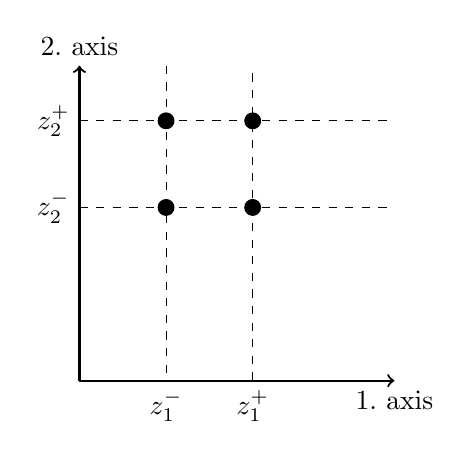
\begin{tikzpicture}
\draw[->, thick] (0,0) --(4,0) node[below] {1. axis};
\draw[->, thick] (0,0) --(0,4) node[above] {2. axis};
\draw[dashed] (1.1,4) --  (1.1,0) node[below] {$z_1^-$} ;
\draw[dashed] (2.2,0) node[below] {$z_1^+$} -- (2.2,4) ;
\draw[dashed] (0,2.2) node[left] {$z_2^-$} -- (4,2.2);
\draw[dashed] (0,3.3)  node[left] {$z_2^+$}-- (4,3.3);
\draw[fill=black] (1.1,2.2) circle (0.1);
\draw[fill=black] (2.2,2.2) circle (0.1);
\draw[fill=black] (2.2,3.3) circle (0.1);
\draw[fill=black] (1.1,3.3) circle (0.1);
\end{tikzpicture}
\caption{A hypercupe in 2 dimensions encapsulated by $(z_1^-, z_2^-)$, $(z_1^+, z_2^-)$, $(z_1^-, z_2^+)$, and $(z_1^+, z_2^+)$.}\label{xminus_xplus}
\end{figure}
Lad $y_1, \dots, y_{2^n}$ være de korresponderende y-værdier for hjørnerne i hyperkuben. Så kan man skrive interpolationsoverfladen som
\begin{equation}
f(z)=f((z_1, \dots, z_n))=\sum_{J\subseteq \{1,\dots, n\}} a_J \prod_{j\in J} z_j \label{nlinear_interpolation}
\end{equation}
hvor 
\begin{equation}
\begin{pmatrix}
a_{\emptyset}\\
a_{\{1\}}\\
\vdots\\
a_{\{1, \dots, n\}}
\end{pmatrix}=\begin{pmatrix}
\vec{v}(z_1^{-},z_2^-, \dots, z_n^-)\\
\vec{v}(z_1^{+},z_2^-, \dots, z_n^-)\\
\vdots\\
\vec{v}(z_1^{+},z_2^+, \dots, z_n^+)\\
\end{pmatrix}^{-1}
\begin{pmatrix}
y_1\\
y_2\\
\vdots\\
y_{2^n}
\end{pmatrix}\label{a_solution}
\end{equation}
hvor
\begin{equation*}
\vec{v}(w_1, \dots, w_n)=\begin{pmatrix}
1 & w_1 & w_2 & \dots & w_n & w_1w_2 & w_1w_3 & \dots & \prod_{i=1}^nw_i
\end{pmatrix}.
\end{equation*}
Det gør at hvert $a$ i \eqref{nlinear_interpolation} kan skrives som en linearkombination af $y_i$'er, og dermed kan de $k$ ligninger i \eqref{integral_equations} skrives som en linearkombinationer af $y_1, \dots, y_k$. Med andre ord kan \eqref{integral_equations} (formodentlig) løses entydigt. Hvordan hyperkuberne skal lægges er illustreret i 2 dimensioner i Figur \ref{hypercubes_placement}. 
\begin{figure}
\centering
\begin{tikzpicture}
\node[anchor=east] at (-0.5,0){
\begin{tikzpicture}
\node[above] at (2.5,4) {\Large (A)};
\draw (1,1) rectangle (2,2);
\draw (2,2) rectangle (3,3);
\draw (3,3) rectangle (4,4);
\draw (1,2) rectangle (2,3);
\draw (2,3) rectangle (3,4);
\draw (2,1) rectangle (3,2);
\draw (3,2) rectangle (4,3);
\draw (1,3) rectangle (2,4);
\draw (3,1) rectangle (4,2);
\end{tikzpicture}};
\node[anchor=west] at (1.5,0) {
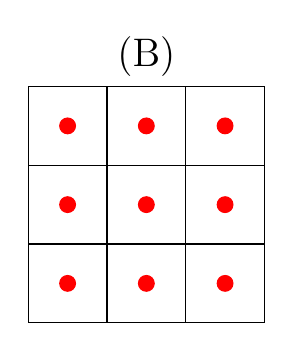
\begin{tikzpicture}
\node[above] at (2.5,4) {\Large (B)};
\draw (1,1) rectangle (2,2);
\draw (2,2) rectangle (3,3);
\draw (3,3) rectangle (4,4);
\draw (1,2) rectangle (2,3);
\draw (2,3) rectangle (3,4);
\draw (2,1) rectangle (3,2);
\draw (3,2) rectangle (4,3);
\draw (1,3) rectangle (2,4);
\draw (3,1) rectangle (4,2);
\foreach \x in {1.5,2.5,3.5}
\foreach \y in {1.5,2.5,3.5}
{
\draw[fill=red, color=red] (\x,\y) circle (0.1);
}
\end{tikzpicture}
};
\node[anchor=east] at (-0.5,-5){
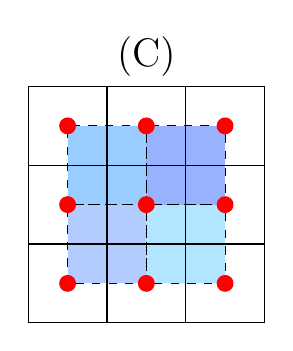
\begin{tikzpicture}
\node[above] at (2.5,4) {\Large (C)};
\fill[color=blue1] (1.5, 1.5) rectangle (2.5,2.5);
\fill[color=blue2] (1.5, 2.5) rectangle (2.5,3.5);
\fill[color=blue3] (2.5, 1.5) rectangle (3.5,2.5);
\fill[color=blue4] (2.5, 2.5) rectangle (3.5,3.5);
\foreach \x in {1.5,2.5}
\foreach \y in {1.5,2.5}
{
\draw[dashed] (\x, \y) rectangle (\x+1,\y+1);
}

\draw (1,1) rectangle (2,2);
\draw (2,2) rectangle (3,3);
\draw (3,3) rectangle (4,4);
\draw (1,2) rectangle (2,3);
\draw (2,3) rectangle (3,4);
\draw (2,1) rectangle (3,2);
\draw (3,2) rectangle (4,3);
\draw (1,3) rectangle (2,4);
\draw (3,1) rectangle (4,2);
\foreach \x in {1.5,2.5,3.5}
\foreach \y in {1.5,2.5,3.5}
{
\draw[fill=red, color=red] (\x,\y) circle (0.1);
}
\end{tikzpicture}};
\node[anchor=west] at (1.5, -5) {
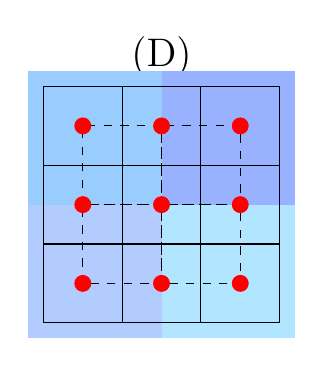
\begin{tikzpicture}
\node[above] at (2.5,4) {\Large (D)};
\fill[color=blue1] (0.8, 0.8) rectangle (2.5,2.5);
\fill[color=blue2] (0.8, 2.5) rectangle (2.5,4.2);
\fill[color=blue3] (2.5, 0.8) rectangle (4.2,2.5);
\fill[color=blue4] (2.5, 2.5) rectangle (4.2,4.2);
\foreach \x in {1.5,2.5}
\foreach \y in {1.5,2.5}
{
\draw[dashed] (\x, \y) rectangle (\x+1,\y+1);
}

\draw (1,1) rectangle (2,2);
\draw (2,2) rectangle (3,3);
\draw (3,3) rectangle (4,4);
\draw (1,2) rectangle (2,3);
\draw (2,3) rectangle (3,4);
\draw (2,1) rectangle (3,2);
\draw (3,2) rectangle (4,3);
\draw (1,3) rectangle (2,4);
\draw (3,1) rectangle (4,2);
\foreach \x in {1.5,2.5,3.5}
\foreach \y in {1.5,2.5,3.5}
{
\draw[fill=red, color=red] (\x,\y) circle (0.1);
}
\end{tikzpicture}};
\end{tikzpicture}
\caption{(A) viser faktorerne i $\mathcal F$, når der er tale om et grid af endelige faktorlevels med positivt lebesguemål (i $\mathbb R^2$). (B) viser midtpunkterne. (C) viser de 4 interpolationsflader der kan laves af de 9 punkter.  (D) viser ekstrapoleringen af de 4 interpolationsområder som potentialt går ud i hele $\mathbb R^2$.
}\label{hypercubes_placement}
\end{figure}


\begin{figure}
\centering
\begin{tikzpicture}
\node[anchor=east] at (-0.5,0){
\begin{tikzpicture}
\node[above] at (2,3) {\Large (A)};
\draw (1,1) rectangle (2,2);
\draw (2,2) rectangle (3,3);
\draw (1,2) rectangle (2,3);
\draw (2,1) rectangle (3,2);
\draw[fill=black] (1,1) circle (0.12);
\draw[ultra thick] (1,1.2) -- (1,1.9);
\draw[ultra thick] (1,2.1) -- (1,2.9);
\draw[ultra thick] (1.2,1) -- (1.9,1);
\draw[ultra thick] (2.1,1) -- (2.9,1);
\end{tikzpicture}};
\node[anchor=west] at (1.5,0) {
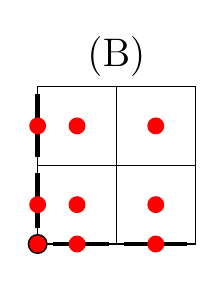
\begin{tikzpicture}
\node[above] at (2,3) {\Large (B)};
\draw (1,1) rectangle (2,2);
\draw (2,2) rectangle (3,3);
\draw (1,2) rectangle (2,3);
\draw (2,1) rectangle (3,2);
\draw[fill=black] (1,1) circle (0.12);
\draw[ultra thick] (1,1.2) -- (1,1.9);
\draw[ultra thick] (1,2.1) -- (1,2.9);
\draw[ultra thick] (1.2,1) -- (1.9,1);
\draw[ultra thick] (2.1,1) -- (2.9,1);
\foreach \x in {1,1.5,2.5}
\foreach \y in {1,1.5,2.5}
{
\draw[fill=red, color=red] (\x,\y) circle (0.1);
}
\end{tikzpicture}
};
\node[anchor=east] at (-0.5,-5){
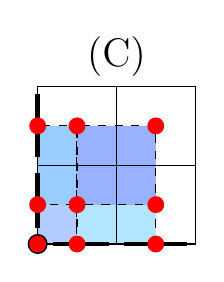
\begin{tikzpicture}
\node[above] at (2,3) {\Large (C)};
\draw[dashed, fill=blue1] (1,1) rectangle (1.5,1.5);
\draw[dashed, fill=blue2] (1,1.5) rectangle (1.5,2.5);
\draw[dashed, fill=blue3] (1.5,1) rectangle (2.5,1.5);
\draw[dashed, fill=blue4] (1.5,1.5) rectangle (2.5,2.5);
\draw (1,1) rectangle (2,2);
\draw (2,2) rectangle (3,3);
\draw (1,2) rectangle (2,3);
\draw (2,1) rectangle (3,2);
\draw[fill=black] (1,1) circle (0.12);
\draw[ultra thick] (1,1.2) -- (1,1.9);
\draw[ultra thick] (1,2.1) -- (1,2.9);
\draw[ultra thick] (1.2,1) -- (1.9,1);
\draw[ultra thick] (2.1,1) -- (2.9,1);
\foreach \x in {1,1.5,2.5}
\foreach \y in {1,1.5,2.5}
{
\draw[fill=red, color=red] (\x,\y) circle (0.1);
}
\end{tikzpicture}};
\node[anchor=west] at (1.5, -5) {
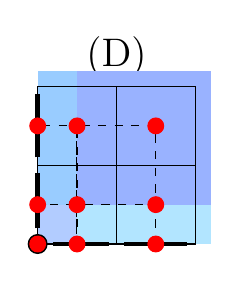
\begin{tikzpicture}
\node[above] at (2,3) {\Large (D)};
\fill[color=blue2] (1,1.5) rectangle (1.5,3.2);
\fill[color=blue3] (1.5,1) rectangle (3.2,1.5);
\fill[color=blue4] (1.5,1.5) rectangle (3.2,3.2);
\draw[dashed, fill=blue1] (1,1) rectangle (1.5,1.5);
\draw[dashed, fill=blue2] (1,1.5) rectangle (1.5,2.5);
\draw[dashed, fill=blue3] (1.5,1) rectangle (2.5,1.5);
\draw[dashed, fill=blue4] (1.5,1.5) rectangle (2.5,2.5);

\draw (1,1) rectangle (2,2);
\draw (2,2) rectangle (3,3);
\draw (1,2) rectangle (2,3);
\draw (2,1) rectangle (3,2);
\draw[fill=black] (1,1) circle (0.12);
\draw[ultra thick] (1,1.2) -- (1,1.9);
\draw[ultra thick] (1,2.1) -- (1,2.9);
\draw[ultra thick] (1.2,1) -- (1.9,1);
\draw[ultra thick] (2.1,1) -- (2.9,1);
\foreach \x in {1,1.5,2.5}
\foreach \y in {1,1.5,2.5}
{
\draw[fill=red, color=red] (\x,\y) circle (0.1);
}
\end{tikzpicture}};
\end{tikzpicture}
\caption{(A) viser faktorerne i $\mathcal F$, når der er tale om et endeligt grid af faktorlevels hvor der dog er punkter og linjer med positivt mål (markeret med sort prik og fed linje, hhv.). (B) viser midtpunkterne. (C) viser de 4 interpolationsflader der kan laves af de 9 punkter.  (D) viser ekstrapoleringen af de 4 interpolationsområder som potentialt går ud i hele $\mathbb R^2$. Læg mærke til at y-værdien i nedre venstre hjørne er kendt, og at der derfor ikke er grund til at opstille integralligningen for den.
}\label{hypercubes_placement2}
\end{figure}

\begin{figure}
\centering
\begin{tikzpicture}
\node[anchor=center] at (-4.5,0){
\begin{tikzpicture}
\node[above] at (2,3.5) {\Large (A)};
\draw (1,1) rectangle (2,2);
\draw[dashed] (1,2) -- (1,3.5);
\draw[dashed] (2,2) -- (2,3.5);
\draw[dashed] (2,1) -- (3.5,1);
\draw[dashed] (2,2) -- (3.5,2);
\draw[dashed, ultra thick] (1,2.1) -- (1,3.5);
\draw[ultra thick] (1,1.1) -- (1,1.9);
\end{tikzpicture}};
\node[anchor=center] at (0,0){
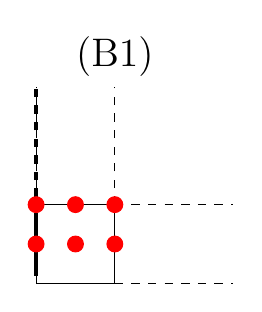
\begin{tikzpicture}
\node[above] at (2,3.5) {\Large (B1)};
\draw (1,1) rectangle (2,2);
\draw[dashed] (1,2) -- (1,3.5);
\draw[dashed] (2,2) -- (2,3.5);
\draw[dashed] (2,1) -- (3.5,1);
\draw[dashed] (2,2) -- (3.5,2);
\draw[dashed, ultra thick] (1,2.1) -- (1,3.5);
\draw[ultra thick] (1,1.1) -- (1,1.9);
\draw[fill=red, color=red] (1,1.5) circle (0.1);
\draw[fill=red, color=red] (1,2) circle (0.1);
\draw[fill=red, color=red] (1.5,2) circle (0.1);
\draw[fill=red, color=red] (2,2) circle (0.1);
\draw[fill=red, color=red] (2,1.5) circle (0.1);
\draw[fill=red, color=red] (1.5,1.5) circle (0.1);
\end{tikzpicture}};
\node[anchor=center] at (4.5, 0) {
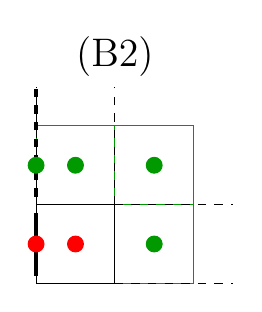
\begin{tikzpicture}
\node[above] at (2,3.5) {\Large (B2)};
\draw[color=gron] (2,1) rectangle (3,2);
\draw[color=gron] (2,2) rectangle (3,3);
\draw[color=gron] (1,2) rectangle (2,3);
\draw (1,1) rectangle (2,2);
\draw[dashed] (1,2) -- (1,3.5);
\draw[dashed] (2,2) -- (2,3.5);
\draw[dashed] (2,1) -- (3.5,1);
\draw[dashed] (2,2) -- (3.5,2);
\draw[dashed, ultra thick] (1,2.1) -- (1,3.5);
\draw[ultra thick] (1,1.1) -- (1,1.9);
\draw[fill=red, color=red] (1,1.5) circle (0.1);
\draw[fill=gron, color=gron] (1,2.5) circle (0.1);
\draw[fill=gron, color=gron] (1.5,2.5) circle (0.1);
\draw[fill=gron, color=gron] (2.5,2.5) circle (0.1);
\draw[fill=gron, color=gron] (2.5,1.5) circle (0.1);
\draw[fill=red, color=red] (1.5,1.5) circle (0.1);
\end{tikzpicture}};

\node[anchor=center] at (-4.5,-4){
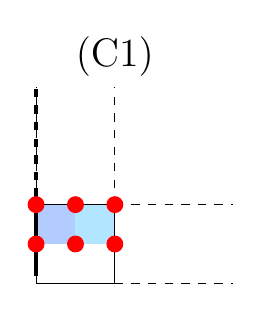
\begin{tikzpicture}
\node[above] at (2,3.5) {\Large (C1)};
\fill[color=blue1] (1,1.5) rectangle (1.5,2);
\fill[color=blue3] (1.5,1.5) rectangle (2,2);
\draw (1,1) rectangle (2,2);
\draw[dashed] (1,2) -- (1,3.5);
\draw[dashed] (2,2) -- (2,3.5);
\draw[dashed] (2,1) -- (3.5,1);
\draw[dashed] (2,2) -- (3.5,2);
\draw[dashed, ultra thick] (1,2.1) -- (1,3.5);
\draw[ultra thick] (1,1.1) -- (1,1.9);
\draw[fill=red, color=red] (1,1.5) circle (0.1);
\draw[fill=red, color=red] (1,2) circle (0.1);
\draw[fill=red, color=red] (1.5,2) circle (0.1);
\draw[fill=red, color=red] (2,2) circle (0.1);
\draw[fill=red, color=red] (2,1.5) circle (0.1);
\draw[fill=red, color=red] (1.5,1.5) circle (0.1);
\end{tikzpicture}};

\node[anchor=center] at (0,-4){
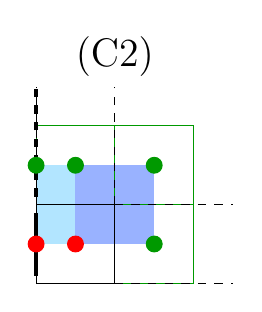
\begin{tikzpicture}
\node[above] at (2,3.5) {\Large (C2)};
\fill[color=blue3] (1,1.5) rectangle (1.5,2.5);
\fill[color=blue4] (1.5,1.5) rectangle (2.5,2.5);
\draw[color=gron] (2,1) rectangle (3,2);
\draw[color=gron] (2,2) rectangle (3,3);
\draw[color=gron] (1,2) rectangle (2,3);
\draw (1,1) rectangle (2,2);
\draw[dashed] (1,2) -- (1,3.5);
\draw[dashed] (2,2) -- (2,3.5);
\draw[dashed] (2,1) -- (3.5,1);
\draw[dashed] (2,2) -- (3.5,2);
\draw[dashed, ultra thick] (1,2.1) -- (1,3.5);
\draw[ultra thick] (1,1.1) -- (1,1.9);
\draw[fill=red, color=red] (1,1.5) circle (0.1);
\draw[fill=gron, color=gron] (1,2.5) circle (0.1);
\draw[fill=gron, color=gron] (1.5,2.5) circle (0.1);
\draw[fill=gron, color=gron] (2.5,2.5) circle (0.1);
\draw[fill=gron, color=gron] (2.5,1.5) circle (0.1);
\draw[fill=red, color=red] (1.5,1.5) circle (0.1);
\end{tikzpicture}};

\node[anchor=center] at (4.5,-4){
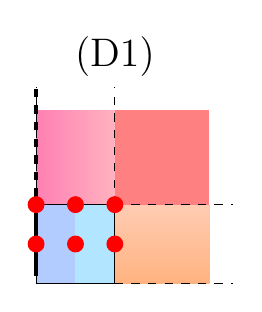
\begin{tikzpicture}
\node[above] at (2,3.5) {\Large (D1)};
\fill[color=blue1] (1,1) rectangle (1.5,2);
\fill[color=blue3] (1.5,1) rectangle (2,2);
\fill[left color=red1, right color=red2] (1,2) rectangle (2,3.2);
\fill[bottom color=red3, top color=red4] (2,1) rectangle (3.2,2);
\fill[color=red5] (2,2) rectangle (3.2,3.2);
\draw (1,1) rectangle (2,2);
\draw[dashed] (1,2) -- (1,3.5);
\draw[dashed] (2,2) -- (2,3.5);
\draw[dashed] (2,1) -- (3.5,1);
\draw[dashed] (2,2) -- (3.5,2);
\draw[dashed, ultra thick] (1,2.1) -- (1,3.5);
\draw[ultra thick] (1,1.1) -- (1,1.9);
\draw[fill=red, color=red] (1,1.5) circle (0.1);
\draw[fill=red, color=red] (1,2) circle (0.1);
\draw[fill=red, color=red] (1.5,2) circle (0.1);
\draw[fill=red, color=red] (2,2) circle (0.1);
\draw[fill=red, color=red] (2,1.5) circle (0.1);
\draw[fill=red, color=red] (1.5,1.5) circle (0.1);
\end{tikzpicture}};

\node[anchor=center] at (-4.5,-8){
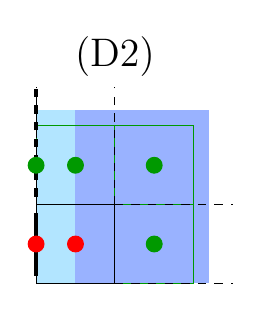
\begin{tikzpicture}
\node[above] at (2,3.5) {\Large (D2)};
\fill[color=blue3] (1,1) rectangle (1.5,3.2);
\fill[color=blue4] (1.5,1) rectangle (3.2,3.2);
\draw[color=gron] (2,1) rectangle (3,2);
\draw[color=gron] (2,2) rectangle (3,3);
\draw[color=gron] (1,2) rectangle (2,3);
\draw (1,1) rectangle (2,2);
\draw[dashed] (1,2) -- (1,3.5);
\draw[dashed] (2,2) -- (2,3.5);
\draw[dashed] (2,1) -- (3.5,1);
\draw[dashed] (2,2) -- (3.5,2);
\draw[dashed, ultra thick] (1,2.1) -- (1,3.5);
\draw[ultra thick] (1,1.1) -- (1,1.9);
\draw[fill=red, color=red] (1,1.5) circle (0.1);
\draw[fill=gron, color=gron] (1,2.5) circle (0.1);
\draw[fill=gron, color=gron] (1.5,2.5) circle (0.1);
\draw[fill=gron, color=gron] (2.5,2.5) circle (0.1);
\draw[fill=gron, color=gron] (2.5,1.5) circle (0.1);
\draw[fill=red, color=red] (1.5,1.5) circle (0.1);
\end{tikzpicture}};

\end{tikzpicture}
\caption{(A) viser faktorerne i $\mathcal F$, når der er tale om et grid af faktorlevels hvor der er linjer med positivt mål og faktorniveauer der breder sig ud mod uendelig (markeret med fed linje og stiplet linje, hhv.). (B1) viser en metode for midtpunkterne, mens (B2) viser en anden. I (B2) er der også sat markeringer af et pseudo-område for (B2). (D1) og (D2) viser, hvad vi ser som den mest naturlige måde at udvide interpolationsfladerne. I (D1) angiver det store røde felt at interpolationsværdien bliver sat til konstanten $r(f)$. De to gradientfelter (hhv. orange og lyserød) indikerer at interpolationsværdien bliver udregnet ved at projicere ned på kanten af den endelige hyperkube. 
}\label{hypercubes_placement3}
\end{figure}
\subsubsection{Løsning af Integralsystem}
Vi løser nu \eqref{integral_equations}. Vi ser fra \eqref{nlinear_interpolation} at vi bør integrere
\begin{align}
&\int_{[z_1^-, z_1^+]\times \cdots \times [ z_n^-,z_n^+]}  z_1\cdot z_2\cdots z_m \textup{ d}(z_1, \dots, z_n)\nonumber\\
&=\int_{[z_2^-, z_2^+]\times \cdots \times [ z_n^-,z_n^+]} \frac{1}{2}\Bigl(\bigl(z_1^+\bigr)^2-\bigl(z_1^-\bigr)^2\Bigr)z_2\cdots z_m  \textup{ d}(z_2, \dots, z_n)\nonumber\\
&=\cdots\nonumber\\
&=\frac{1}{2^m}\prod_{i=1}^m \Bigl(\bigl(z_i^+\bigr)^2-\bigl(z_i^-\bigr)^2\Bigr)\int_{[z_{m+1}^-, z_{m+1}^+]\times \cdots \times [ z_n^-,z_n^+]}  1 \textup{ d}(z_1, \dots, z_n)\nonumber\\
&=\frac{1}{2^m}\prod_{i=1}^m \Bigl(\bigl(z_i^+\bigr)^2-\bigl(z_i^-\bigr)^2\Bigr)\prod_{i={m+1}}^n \bigl(z_i^+-z_i^-\bigr)\label{integral_prodz_intervals}
\end{align}
under antagelsen at $z_i^+>z_i^-$. I det mere generelle tilfælde, hvor $z_i^+ \geq z_i^-$ antager vi at når $z_i^+=z_i^-$ integrerer vi med hensyn til dirac-målet koncentreret i $z_i^{+}$. I så fald bliver \eqref{integral_prodz_intervals} i stedet
\begin{gather} 
H\bigl([(z_1^-, z_1^+),\dots, ( z_n^-,z_n^+)], \{1, \dots, m\}\bigr):=\nonumber\\
\prod_{i=1, z_i^{-}\neq z_i^+}^m \Bigl(\frac{1}{2}\bigl(z_i^+\bigr)^2-\frac{1}{2}\bigl(z_i^-\bigr)^2\Bigr)\prod_{i=1,z_i^{-}= z_i^+ } z_i^+ \prod_{i={m+1},z_i^{-}\neq z_i^+ }^n \bigl(z_i^+-z_i^-\bigr)\label{integral_prodz}
\end{gather}
Nu udvider vi notationen lidt. Lad 
\begin{equation}
\textup{mid}(f)=(\textup{mid}_1(f_1), \dots, \textup{mid}_n(f_n))
\end{equation}
være midtpunktet for faktorniveau $f=(f_1, \dots, f_n)\in \mathcal F$. Vi antager at $\mathcal F$ er et grid, dvs.
\begin{equation}
\mathcal F= \Bigl\{\begin{lgathered}[t] [a_1^-(j_1), a_1^+(j_1)]\times \cdots \times [a_n^-(j_n), a_n^+(j_n)]:\\
j_1\in \{1, \dots, k_1\}, \dots j_n\in \{1, \dots, k_n\}\Bigr\}\end{lgathered}
\end{equation}
hvor $a_i^{\pm}(j)$ er passende konstanter i $\mathbb R \cup \{-\infty, \infty\}$, der opfylder
\begin{equation*}
a_i^+(j)=a_i^-(j+1), \quad j=1, \dots, k_i-1
\end{equation*}
Per definition af midpoint ved vi
\begin{equation}
a_i^-(j)\leq \textup{mid}_i\bigl([a_i^-(j), a_i^+(j)]\bigr) \leq a_i^+(j)
\end{equation}
Vi forkorter notationen yderligere med 
\begin{equation*}
z(i,j)=\textup{mid}_i\bigl([a_i^-(j), a_i^+(j)]\bigr).
\end{equation*}
og dermed kan et midtpunkt skrives som
\begin{equation}
\bigl(z(1,j_1), z(2,j_2), \dots, z(n, j_n)\bigr)
\end{equation}
for passende $j_1\dots, j_n $. En interpolationsflade (noteret $f$ i \eqref{nlinear_interpolation}), kan nu skrives mere præcist som
\begin{align}
h^{j_1, \dots, j_n}(z)=\sum_{J\subseteq\{1, \dots, n\}} a_J(j_1, \dots, j_n) \prod_{j\in J} z_j \label{more_explicit_interpolation}
\end{align}
for $j_i\in \{1, \dots, k_{i}-1\}$, hvilket giver $(k_1-1)\cdots (k_n-1)$ forskellige interpolationsflader. Interpolationsfladen i  \eqref{more_explicit_interpolation} gælder umiddelbart kun for $z$ i mængden
\begin{align}
& [z(1,j_1), z(1,j_1+1)]\times \cdots \times [z(n,j_n), z(n,j_n+1)]
\end{align}
Dog udvider vi ofte denne mængde, se Figur \ref{hypercubes_placement}, \ref{hypercubes_placement2} og \ref{hypercubes_placement3}. For at løse ligningssystemet \eqref{integral_equations} med (B2)-midpoints sætter vi
\begin{align}
\tilde z(i,j) =\begin{cases} a_i^-(1)\quad &\textup{hvis } j=1, a_i^-(j)>-\infty\\
a_i^+(1)-\bigl(a_i^+(2)-a_i^-(2)\bigr)&\textup{hvis } j=1, a_i^-(j)=-\infty\\
a_i^+(k_j)\quad &\textup{hvis } j=k_j, a_i^+(k_j)<\infty\\
a_i^+(k_j)+\bigl(a_i^+(k_j-1)-a_i^-(k_j-1)\bigr)&\textup{hvis } j=k_j, a_i^+(j)=\infty\\
z(i,j) & \textup{ellers.}
\end{cases}
\end{align}
og lader \eqref{more_explicit_interpolation} være gældende for $z$ i mængden
\begin{equation*}
[\tilde z(1,j_1), \tilde z(1,j_1+1)]\times \cdots \times [\tilde z(n,j_n), \tilde z(n,j_n+1)].
\end{equation*}
I integralet i \eqref{integral_equations} skal vi integrere over $f$. Hvis vi bruger (B2) er det nemmest at formulere integralet ved at justere $a_i^{\pm}$'erne. Det gøres med
\begin{align*}
\tilde a_i^-(j) =\begin{cases} 
a_i^+(1)-\bigl(a_i^+(2)-a_i^-(2)\bigr)&\textup{hvis } j=1, a_i^-(j)=-\infty\\
a_i^-(j) & \textup{ellers.}
\end{cases}
\end{align*}
og
\begin{align*}
\tilde a_i^+(j) =\begin{cases} 
a_i^+(k_j)+\bigl(a_i^+(k_j-1)-a_i^-(k_j-1)\bigr)&\textup{hvis } j=k_j, a_i^+(j)=\infty\\
a_i^+(j) & \textup{ellers.}
\end{cases}
\end{align*}
For at gøre notationen nemmere i kanterne af grid'et, sættes også
\begin{align}
h^{j_1, \dots, j_n}&=h^{(j_1 \wedge k_1-1)\vee 1, \dots, (j_n \wedge k_n-1)\vee 1},\\
a_J({j_1, \dots, j_n})&=a_J\bigl((j_1 \wedge k_1-1)\vee 1, \dots, (j_n \wedge k_n-1)\vee 1\bigr)
\end{align}
for $ j_i\in \{0, \dots, k_i\}, i=1, \dots, n, J\subseteq \{1, \dots, n\}$

Bemærk at et $f\in\mathcal F$ er kendetegnet ved $j_1,\dots, j_n$. Da kan vi skrive ligningssystemet \eqref{integral_equations} som $k$ ligninger, der hver består af en sum af $2^n$ integraler.
\begin{align}
r(j_1,\dots, j_n)&=\begin{lgathered}[t]\int_{[\tilde a_1^-(j_1), z(1,j_1)]\times \cdots \times [\tilde a_n^-(j_n),  z(n,j_n)]} \hspace{-2cm} h^{j_1-1, \dots, j_n-1}(z) \textup{ d}z\\
+\int_{[z(1,j_1), \tilde a_1^+(j_1)]\times [\tilde a_2^-(j_2), z(2,j_2)]\times \cdots \times [\tilde a_n^-(j_n),  z(n,j_n)]} \hspace{-4cm}h^{j_1,j_2-1 \dots, j_n-1}(z) \textup{ d}z\\
\vdots\\
+\int_{[z(1,j_1), \tilde a_1^+(j_1), ]\times \cdots \times [z(n,j_n), \tilde a_n^+(j_n)]} 
\hspace{-2cm}h^{j_1,j_2 \dots, j_n}(z) \textup{ d}z
\end{lgathered}\label{integral_equations_by_js}
\end{align}
Ved at bruge $H$ fra tidligere kan vi sætte
\begin{align}
&\int_{[\tilde a_1^-(j_1), z(1,j_1)]\times \cdots \times [\tilde a_n^-(j_n),  z(n,j_n)]} \hspace{-2cm} h^{j_1-1, \dots, j_n-1}(z) \textup{ d}z\nonumber\\
&=\sum_{J\subseteq\{1, \dots, n\}}\Bigl( \begin{lgathered}[t]a_J(j_1-1, \dots, j_n-1)\\
\cdot H\bigl([(\tilde a_1^-(j_1), z(1,j_1)), \dots, (\tilde a_n^-(j_n), z(n,j_n)], J\bigr)\Bigr)\end{lgathered}\label{integral_computation_before_matrices}
\end{align}
Definer nu
\begin{equation}
\mathbf{V}(j_1, \dots, j_n)=\begin{pmatrix}
\vec{v}(z(1,j_1),z(2,j_2), \dots, z(n,j_n))\\
\vec{v}(z(1,j_1+1),z(2,j_2), \dots, z(n,j_n))\\
\vec{v}(z(1,j_1),z(2,j_2+1), \dots, z(n,j_n))\\
\vdots\\
\vec{v}(z(1,j_1+1),z(2,j_2+1), \dots, z(n,j_n+1))\\
\end{pmatrix}.
\end{equation}
med 
\begin{equation}
\mathbf{V}({j_1, \dots, j_n})=\mathbf{V}\bigl((j_1 \wedge [k_1-1])\vee 1, \dots, (j_n \wedge [k_n-1])\vee 1\bigr)
\end{equation}
for $ j_i\in \{0, \dots, k_i\}, i=1, \dots, n$, samt
\begin{equation}
\mathbf{y}(j_1, \dots, j_n)=\begin{pmatrix}
y(j_1,j_2, \dots, j_n)\\
y(j_1+1, j_2,\dots, j_n)\\
\vdots\\
y(j_1+1, \dots, j_n+1)
\end{pmatrix}
\end{equation}
for $j_i \in \{1,\dots, k_i-1\}, i=1, \dots, n$. Vi definerer
\begin{equation}
\mathbf y(j_1, \dots, j_n)=\mathbf y \bigl((j_1 \wedge [k_1-1])\vee 1, \dots, (j_n \wedge [k_n-1])\vee 1\bigr)
\end{equation}
for generelle $j_i \in \{0,\dots, k_i\}, i=1, \dots, n$.

Vi fortolker $y(j_1, \dots, j_n)$ som interpolationens y-værdi i $(z(1,j_1), \dots, z(n,j_n))$. Altså er $\mathbf {y}$ vektoren af y-værdier, der indgår i $h^{j_1, \dots, j_n}$. Indsat i \eqref{integral_computation_before_matrices} giver det
\begin{equation}
\sum_{J\subseteq\{1, \dots, n\}}\Bigl( \begin{lgathered}[t]\mathbf{e}_J^T \mathbf{V}(j_1-1, \dots, j_n-1)^{-1} \mathbf{y}(j_1-1, \dots, j_n-1)\\
\cdot H\bigl([(\tilde a_1^-(j_1), z(1,j_1)), \dots, (\tilde a_n^-(j_n), z(n,j_n)], J\bigr)\Bigr)\end{lgathered}\label{integral_computation_matrix1}
\end{equation}
hvor $\mathbf{e}_J$ er en vektor af 0'er på nær et 1-tal i den indgang der svarer til den koordinat der svarer til $J$. Hvis vi definerer vektoren af længde $2^n$ 
\begin{align}
\mathbf{H}\bigl(&[(\tilde a_1^-(j_1), z(1,j_1)), \dots, (\tilde a_n^-(j_n), z(n,j_n)]\bigr)\\
&=\begin{pmatrix}
H\bigl([(\tilde a_1^-(j_1), z(1,j_1)), \dots, (\tilde a_n^-(j_n), z(n,j_n)], \emptyset \bigr)\\
H\bigl([(\tilde a_1^-(j_1), z(1,j_1)), \dots, (\tilde a_n^-(j_n), z(n,j_n)], \{1\} \bigr)\\
\vdots \\
H\bigl([(\tilde a_1^-(j_1), z(1,j_1)), \dots, (\tilde a_n^-(j_n), z(n,j_n)], \{1, \dots, n\} \bigr)
\end{pmatrix}
\end{align}
kan vi skrive \eqref{integral_computation_matrix1} som
\begin{equation}
\Bigl[\begin{lgathered}[t] \mathbf{H}\bigl([(\tilde a_1^-(j_1), z(1,j_1)), \dots, (\tilde a_n^-(j_n), z(n,j_n)]\bigr)^T\\
\cdot \mathbf{V}(j_1-1, \dots, j_n-1)^{-1} \Bigr] \mathbf{y}(j_1-1, \dots, j_n-1) \end{lgathered}\label{integral_computation_matrix2}
\end{equation}
Vi kan derfor skrive ligningssystemet fra \eqref{integral_equations_by_js} som
\begin{align}
r(j_1, \dots, j_n)&=\Biggl\{\begin{lgathered}[t]\Bigl[\begin{lgathered}[t] \mathbf{H}\bigl([(\tilde a_1^-(j_1), z(1,j_1)), \dots, (\tilde a_n^-(j_n), z(n,j_n)]\bigr)^T\\
\cdot \mathbf{V}(j_1-1, \dots, j_n-1)^{-1} \Bigr] \mathbf{y}(j_1-1, \dots, j_n-1) \end{lgathered}\\
+
\Bigl[\begin{lgathered}[t] \mathbf{H}\bigl([(z(1,j_1), \tilde a_1^+(j_1)), \dots, (\tilde a_n^-(j_n), z(n,j_n)]\bigr)^T\\
\cdot \mathbf{V}(j_1,j_2-1 \dots, j_n-1)^{-1} \Bigr] \mathbf{y}(j_1,j_2-1 \dots, j_n-1)+ \end{lgathered} \\
\vdots\\
+\Bigl[\begin{lgathered}[t] \mathbf{H}\bigl([( z(1,j_1), \tilde a_1^+(j_1)), \dots, (z(n,j_n), \tilde a_n^+(j_n))]\bigr)^T\\
\cdot \mathbf{V}(j_1, \dots, j_n)^{-1} \Bigr] \mathbf{y}(j_1, \dots, j_n) \Biggr\}\end{lgathered}\\
\end{lgathered}\label{integral_computation_matrix3}
\end{align}
Ud fra \eqref{integral_computation_matrix3} kræver det et stykke (trivielt) omrokeringsarbejde at få det på formen
\begin{equation}
\bigl\{r(j_1, \dots, j_n)\bigr\}_{j_i\in\{1, \dots, k_i\}, i=1, \dots, n}=B\bigl\{y(j_1, \dots, j_n)\bigr\}_{j_i\in\{1, \dots, k_i\}, i=1, \dots, n}
\end{equation}
som løses ved at invertere $k\times k$ matricen $B$. Når de $k$ y-værdier er fundet regnes matrix produkterne
\begin{align}
\mathbf{V}(j_1, \dots, j_n)^{-1} \mathbf{y}(j_1, \dots, j_n)
\end{align}
og koefficienterne sættes ind i risk ratio filerne.

\subsection{Multivariate splines}

\begin{figure}
\centering
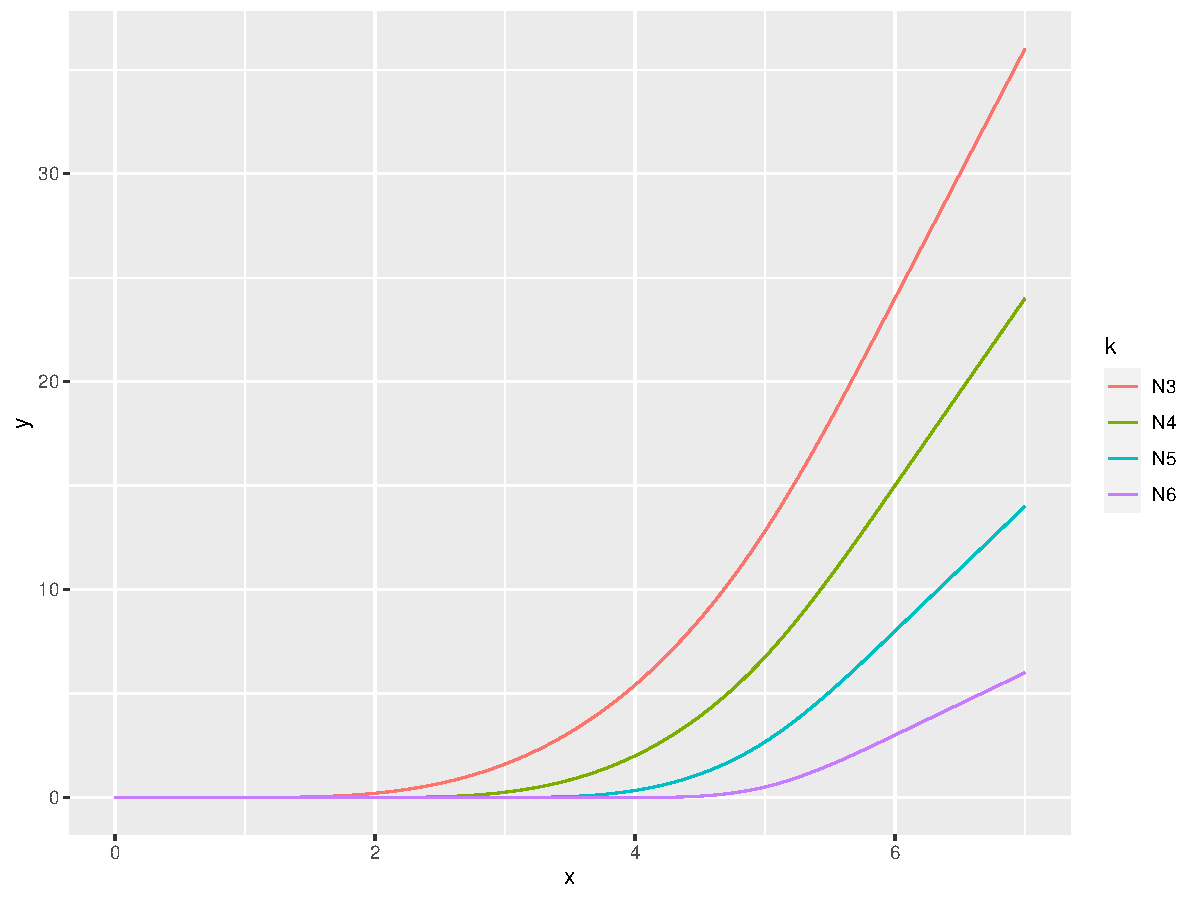
\includegraphics[width=\textwidth]{natural_cubic_splines.pdf}
\caption{For 6 punkter i $\{1,2,3,4,5,6\}$ vises her de De 4 sidste basisfunktioner for natural cubic splines.}\label{natural_cubic_spline}
\end{figure}


I stedet for eksplicit at modellere midtpunkterne mellem stykkerne, kan vi også modellere funktionen direkte. Hvis vi for eksempel tager den naturlige kubiske spline (se Figur \ref{natural_cubic_spline}) har den i en enkelt dimension basis
\begin{align*}
N_1(X)&=1\\, N_2(X)&=X\\
N_{k+2}(X)&=\frac{(X-x_k)_+^3-(X-x_K)_+^3}{x_K-x_k}-\frac{(X-x_{K-1})^3_+-(X-x_K)^3_+}{x_K-x_{K-1}}\\
&=\begin{lgathered}[t]\mathbb{I}(x_{K}\geq X>x_k)\frac{X^3-x_k^3+3Xx_k^2-3X^2x_k}{x_K-x_k}\\
-\mathbb{I}(x_K\geq X>x_{K-1})\frac{X^3-x_{K-1}^3+3Xx_{K-1}^2-3X^2x_{K-1}}{x_K-x_{K-1}}\\
+\mathbb{I}(X>x_K)\frac{-x_k^3+x_K^3+3X(x_k^2-x_K^2)-3X^2(x_k-x_K)}{x_K-x_k}\\
-\mathbb{I}(X>x_K)\frac{-x_{K-1}^3+x_K^3+3X(x_{K-1}^2-x_K^2)-3X^2(x_{K-1}-x_K)}{x_K-x_{K-1}}\\\end{lgathered}\\
&=\begin{lgathered}[t]X^3\mathbb{I}(x_{K}\geq X>x_k) \Bigl(\frac{1}{x_K-x_k}-\frac{\mathbb{I}(X>x_{K-1})}{x_K-x_{K-1}}\Bigr)\\
+X^2\mathbb{I}(x_{K}\geq X>x_k) \Bigl(  \frac{-3x_k}{x_K-x_k}-\mathbb{I}( X>x_{K-1})\frac{-3x_{K-1}}{x_K-x_{K-1}}  \Bigr)\\
+X\mathbb{I}(X>x_k)\Bigl(
           \begin{lgathered}[t]
                        \frac{\mathbb{I}(X\leq x_K) 3x_k^2}{x_K-x_k}-\frac{\mathbb{I}(x_K\geq X>x_{K-1})3x_{K-1}^2}{x_{K}-x_{K-1}}\\
                        +\mathbb{I}(X>x_K) \bigl(-3(x_K+x_k)+3(x_K+x_{K-1})\bigr)
           \Bigr)
 \end{lgathered}\\
 + \mathbb{I}(x_{K}\geq X>x_k)\frac{-x_k^3}{x_K-x_k}-\mathbb{I}(x_{K}\geq X>x_{K-1})\frac{-x_{K-1}^3}{x_K-x_{K-1}}\\
+ \mathbb{I}(X>x_K)\Bigl(\frac{-x_k^3+x_K^3}{x_K-x_{k}}-\frac{-x_{K-1}^3+x_K^3}{x_K-x_{K-1}}\Bigr)
\end{lgathered}
\end{align*}
Hvis vi har flere dimensioner dvs. $X_1, X_2, \dots X_N$ tager vi da basisen
\begin{equation}
\{1\}\cup \{N_k(X_i)\}_{i=1,\dots, N, k=2, \dots, K_i}\cup\Bigl\{N_k(X_i)N_l(X_j)\Bigr\}_{i\neq j\in \{1, \dots, N\}, k=2, \dots, K_i, l=2, \dots, K_j}
\end{equation}
Vi estimerer altså funktionen
\begin{equation*}
g(X_1, \dots, X_N)=\beta_1+\sum_{i=1}^N\sum_{j>i}^N \sum_{k=2}^{K_i}\sum_{l=2}^{K_j} \beta_{ijkl}N_k(X_i)N_l(X_j)+\sum_{i=1}^N\sum_{k=1}^{K_i}\beta_{ik}N_k(X_i)
\end{equation*}
hvor vi som likelihoodfunktion har
\begin{equation*}
r(f)|f| \sim N\Biggl(\int_f g(X_1, \dots, X_N) \textup{ d}(X_1, \dots, X_N), \sigma^2\Biggr)
\end{equation*}
for alle $f\in\mathcal F$. For at reducere overfitningen, bruger vi regulariseringen
\begin{equation}
\lambda \sum_{f\in\mathcal F} \int_f \sum_{i=1}^N \sum_{j=1}^N \Bigl(\frac{\partial g}{\partial X_i\partial X_j}\Bigr)^2  \textup{ d}(X_1, \dots, X_N)\label{regul}
\end{equation}
For $r\neq s$ er den inderste del på formen
\begin{align*}
\frac{\partial g}{\partial X_r\partial X_s} &= \sum_{i=1}^N\sum_{j>i}^N \sum_{k=2}^{K_i}\sum_{j=2}^{K_j} \beta_{ijkl}\frac{\partial }{\partial X_r\partial X_s} N_k(X_i)N_l(X_j)\\
&=\sum_{k=2}^{K_r}\sum_{l=2}^{K_s} \beta_{rskl}N_k'(X_r)N_l'(X_s)
\end{align*}
og for $r= s$ på formen
\begin{align}
\frac{\partial g}{\partial X_r\partial X_r} &= \begin{lgathered}[t]\sum_{i=1}^N\sum_{j>i}^N \sum_{k=2}^{K_i}\sum_{j=2}^{K_j} \beta_{ijkl}\frac{\partial }{\partial X_r\partial X_r} N_k(X_i)N_l(X_j)\\
+\sum_{k=1}^{K_r}\beta_{rk}N_k''(X_r)
\end{lgathered}\\
&=\begin{lgathered}[t] \sum_{i=1}^{r-1} \sum_{k=2}^{K_r}\sum_{l=2}^{K_r} \beta_{irkl} N_k(X_i)N_l''(X_r)\\
+\sum_{j=r+1}^N \sum_{k=2}^{K_r}\sum_{l=2}^{K_r} \beta_{rjkl} N_k''(X_r)N_l(X_j)\\
+\sum_{k=1}^{K_r}\beta_{rk}N_k''(X_r)
\end{lgathered}
\end{align}
%
%Vi skriver da
%\begin{align*}
%\sum_{i=1}^{r-1}& \sum_{k=2}^{K_r}\sum_{l=2}^{K_r} \beta_{irkl} N_k(X_i)N_l''(X_r)+\sum_{j=r+1}^N \sum_{k=2}^{K_r}\sum_{l=2}^{K_r} \beta_{rjkl} N_k''(X_r)N_l(X_j)\\
%&=\sum_{i=1, i\neq r}^{N} \sum_{k=2}^{K_r}\sum_{l=2}^{K_r} \beta_{irkl} N_k(X_i)N_l''(X_r)
%\end{align*}
%med konventionen $\beta_{irkl}=\beta_{rilk}$ når $r>i$. 

Det vil sige at indmaden i \eqref{regul} bliver for $r\neq s$
\begin{align}
\sum_{k_1=2}^{K_r}\sum_{k_2=2}^{K_s}\sum_{l_1=2}^{K_r}\sum_{l_2=2}^{K_s} \beta_{rsk_1l_1}N_{k_1}'(X_r)N_{k_2}'(X_r)N_{l_1}'(X_s)N_{l_2}'(X_s)\beta_{rsk_2l_2} \label{regul_rneqs}
\end{align}
og for $r=s$ bliver den
\begin{align}
&\sum_{j_1=r+1}^N \sum_{k_1=2}^{K_r}\sum_{l_1=2}^{K_{j_1}} \sum_{j_2=r+1}^N \sum_{k_2=2}^{K_r}\sum_{l_2=2}^{K_{j_2}}
 \beta_{rj_1k_1l_1} N_{k_1}''(X_r)N_{l_1}(X_{j_1})  N_{k_2}''(X_r)N_{l_2}(X_{j_2})\beta_{rj_2k_2l_2} \label{regul_reqs_j1j2}\\
 &+\sum_{i_1=1}^{r-1} \sum_{k_1=2}^{K_{i_1}}\sum_{l_1=2}^{K_{r}} \sum_{i_2=1}^{r-1} \sum_{k_2=2}^{K_{i_2}}\sum_{l_2=2}^{K_{r}}
 \beta_{i_1rk_1l_1} N_{k_1}(X_{i_1})N_{l_1}''(X_{r})  N_{k_2}(X_{i_2})N_{l_2}''(X_{r})\beta_{i_2rk_2l_2} \label{regul_reqs_i1i2}\\
   &+ \sum_{k_1=2}^{K_r}\sum_{k_2=2}^{K_r}  \beta_{rk_1} N_{k_1}''(X_r)N_{k_2}''(X_r) \beta_{rk_2} \label{regul_reqs_k1k2}\\
   &+2 \sum_{k_1=2}^{K_r}\sum_{j=r+1}^N\sum_{k_2=2}^{K_r}\sum_{l_2=2}^{K_{j}} \beta_{rk_1} \beta_{rjk_2l_2} N_{k_1}''(X_r)N_{k_2}''(X_r)N_{l_2}(X_j)\label{regul_reqs_k1j}\\
   &+2 \sum_{k_1=2}^{K_r}\sum_{i=1}^{r-1}\sum_{k_2=2}^{K_{i}}\sum_{l_2=2}^{K_{r}} \beta_{rk_1} \beta_{irk_2l_2} N_{k_1}''(X_r)N_{k_2}(X_i)N_{l_2}''(X_r)\label{regul_reqs_k1i}\\
      &+2 \sum_{j=r+1}^N \sum_{k_1=2}^{K_r} \sum_{l_2=2}^{K_{j}} \sum_{i=1}^{r-1}\sum_{k_2=2}^{K_{i}}\sum_{l_2=2}^{K_{r}} \beta_{rjk_1l_1} \beta_{irk_2l_2} N_{k_1}''(X_r)N_{l_1}(X_j)N_{k_2}(X_i)N_{l_2}''(X_r)\label{regul_reqs_k1i}
 %&+2\sum_{j_1=1, j_1\neq r}^N \sum_{k_1=2}^{K_r}\sum_{l_1=2}^{K_{j_1}}\sum_{k_2=2}^{K_r} \beta_{rjkl} N_{k_1}''(X_r)N_{l_1}(X_{j_1})N_{k_2}''(X_r) \beta_{rk_2} \label{regul_reqs_j1}\\
\end{align}

Målet er nu at skrive \eqref{regul} på formen
\begin{equation*}
\lambda \beta^* W \beta.
\end{equation*}
Hvis vi betragter situationen udtrykket \eqref{regul_rneqs} ser vi at vi hvis vi definerer 
\begin{equation*}
\beta_{rs\bullet\bullet}^T=\begin{pmatrix}
\beta_{rs2,2} &\beta_{rs2,3} &\dots & \beta_{rs2,K_s} &\beta_{rs3,2} & \dots & \beta_{rsK_rK_s}
\end{pmatrix}
\end{equation*}
kan vi skrive \eqref{regul_rneqs} som 
\begin{equation*}
\beta_{rs\bullet\bullet}^TW_{rs}\beta_{rs\bullet\bullet}
\end{equation*}
hvor 
\begin{equation}
W_{rs}=\begin{pmatrix}
w_{rs2,2,2,2} & w_{rs2,2,2,3}& \dots & w_{rs2,2,2,K_s} & w_{rs2,2,3,2} &\dots &w_{rs2,2,K_r,K_s}\\
w_{rs2,3,2,2} &  w_{rs2,3,2,3} & \dots &&&&w_{rs2,3,K_r,K_s}\\
\vdots &&\ddots &&&&\vdots\\
w_{rsK_rK_s,2,2}&\dots &&&&&w_{rsK_rK_sK_rK_s}
\end{pmatrix}
\end{equation}
hvor
\begin{equation}
w_{rsk_1,l_1,k_2,l_2}=N_{k_1}'(X_r)N_{l_1}'(X_s)N_{k_2}'(X_r)N_{l_2}'(X_s)
\end{equation}

Lad nu 
\begin{align}
\tilde w_{rsk_1,l_1,k_2,l_2}&= \sum_{f\in \mathcal F} \int_f w_{rsk_1,l_1,k_2,l_2} \textup{ d}(X_1, \dots, X_N)\\
\tilde W_{rs}&=\sum_{f\in \mathcal F} \int_f W_{rs} \textup{ d}(X_1, \dots, X_N)\\
\beta&= \begin{pmatrix}
\beta_1\\
\beta_{1,1}\\
\beta_{1,2}\\
\vdots\\
\beta_{N,K_N}\\
 \beta_{1,2\bullet\bullet}\\
  \vdots\\
   \beta_{N-1,N\bullet\bullet}
\end{pmatrix}
\end{align}
Dimensionen af \(\beta\) er 
\begin{equation*}
1+\sum_{i=1}^N(K_i-1)+\sum_{i=1}^N\sum_{j>i}^N (K_i-1)(K_j-1)
\end{equation*}
For at finde bidraget af $r\neq s$ leddene fra \eqref{regul_rneqs}  i den samlede regularisering, \eqref{regul}, definerer jeg
\begin{align}
\tilde W_1&=\begin{pmatrix}
\bigzero &\rvline &\cdot&\cdot&\cdot&\cdot\\
\hline
\cdot & \rvline& \tilde W_{12} &0 & \dots & 0 \\
\cdot & \rvline&0 & \tilde W_{13} &  & \vdots \\
\cdot &\rvline & \vdots &&\ddots &\\
\cdot & \rvline & 0 &\dots & & \tilde W_{N-1,N}
\end{pmatrix}
\end{align}
og da er regulariseringen fra $r\neq s$ leddene
\begin{equation}
\lambda \beta^T (2\tilde W_1) \beta
\end{equation}
For $r=s$ bliver det mere kompliceret. Når man kigger på leddene i \eqref{regul_reqs_j1j2} ser man at der er for et fast $j_1$ og $j_2$ står tilbage
\begin{align*}
\sum_{k_1=2}^{K_r}&\sum_{l_1=2}^{K_r} \sum_{k_2=2}^{K_r}\sum_{l_2=2}^{K_r}
\beta_{rj_1k_1l_1} N_{k_1}''(X_r)N_{l_1}(X_{j_1})  N_{k_2}''(X_r)N_{l_2}(X_{j_2})\beta_{rj_2k_2l_2}\\
\end{align*}
For $r<j_1, r<j_2$ ses det at være
\begin{equation}
\beta_{rj_1\bullet \bullet}^T W_{(r,j_1),(r,j_2)} \beta_{rj_2\bullet\bullet}
\end{equation}
hvor $W_{(r,j_1), (r,j_2)}$ er matricen
\begin{align}
\begin{pmatrix}
w_{rj_1rj_22,2,2,2} & w_{rj_1rj_22,2,2,3}& \dots & w_{rj_1rj_22,2,2,K_{j_2}}  &\dots &w_{rj_1rj_22,2,K_r,K_{j_2}}\\
w_{rj_1rj_22,3,2,2} &  w_{rj_1rj_22,3,2,3} & \dots &&&w_{rj_1rj_22,3,K_r,K_{j_2}}\\
\vdots &&\ddots &&&\vdots\\
w_{rj_1rj_2K_rK_{j_1},2,2}&\dots &&&&w_{rj_1rj_2K_rK_{j_1}K_rK_{j_2}}
\end{pmatrix}
\end{align}
hvor 
\begin{equation}
w_{rj_1rj_2k_1l_1k_2l_2}=N_{k_1}''(X_r)N_{l_1}(X_{j_1})  N_{k_2}''(X_r)N_{l_2}(X_{j_2})
\end{equation}
Når fx $r>j_1$ er problemet, at der ikke findes en $\beta_{rj_1\bullet\bullet}$. Der findes dog 


Betragt nu \eqref{regul_reqs_j1} for et fast $j_1$. 
\begin{equation}
2 \sum_{k_1=2}^{K_r}\sum_{l_1=2}^{K_{j_1}}\sum_{k_2=2}^{K_r} \beta_{rj_1kl} N_{k_1}''(X_r)N_{l_1}(X_{j_1})N_{k_2}''(X_r) \beta_{rk_2}\label{regul_reqs_fixedj1}
\end{equation}
Lad nu 
\begin{equation}
\beta_{r\bullet}^T=\begin{pmatrix}
\beta_{r2} &\dots & \beta_{rK_r}
\end{pmatrix}=\begin{pmatrix}
\beta_{rj2,1} &\beta_{rj3,1} & \dots & \beta_{rjK_r1}
\end{pmatrix}
\end{equation}
og definer
\begin{align}
&W_{(r,0), (r,j_2)}\nonumber\\
&=\begin{pmatrix}
w_{r0rj_22,1,2,2} & w_{r0rj_22,1,2,3}& \dots & w_{r0rj_22,1,2,K_{j_2}}  &\dots &w_{r0rj_22,1,K_r,K_{j_2}}\\
w_{r0rj_23,1,2,2} &  w_{r0rj_22,1,2,3} & \dots &&&w_{r0rj_22,1,K_r,K_{j_2}}\\
\vdots &&\ddots &&&\vdots\\
w_{r0rj_2K_r1,2,2}&\dots &&&&w_{r0rj_2K_r1K_rK_{j_2}}
\end{pmatrix}\\
&W_{(r,j_1),(r,0)}=W_{(r,0), (r,j_1)}^T
\end{align}
hvor 
\begin{equation}
w_{r0rjk_1,1,k_2,l_2}=N_{k_1}''(X_r)N_{l_1}(X_{j_1})N_{k_2}''(X_r)
\end{equation}
Da kan vi skrive \eqref{regul_reqs_fixedj1} som
\begin{equation}
2\beta_{rj_1\bullet\bullet}^T W_{(r,0),(r,j_1)} \beta_{r\bullet}=\beta_{rj_1\bullet\bullet}^TW_{(r,0),(r,j_1)}\beta_{r\bullet}+\beta_{r\bullet}^T W_{(r,j_1),(r,0)}\beta_{rj_1\bullet\bullet}
\end{equation}

Det sidste led, \eqref{regul_reqs} ses at være
\begin{equation}
\beta_{r\bullet}^T \Bigl\{N_{k_1}''(X_r)N_{k_2}(X_r)\Bigr\}_{k_1,k_2=2, \dots, K_r} \beta_{r\bullet}
\end{equation}
Vi kalder matricen $\Bigl\{N_{k_1}''(X_r)N_{k_2}(X_r)\Bigr\}_{k_1,k_2=2, \dots, K_r}$ for $W_0$. 



For at udtrykke den fulde regularisering, \eqref{regul}, i formen $\beta^TW\beta$ mangler vi kun at få sat 






\end{document}